To motivate our approach, we start  by the continuous time representation of the problem we are addressing.
\subsection{Continuous time formulation}

The purpose of this work is to approximate $\expt{g(\mathbf{X}_T)}$, where $g$ is a certain payoff function and $\mathbf{X}=(X_1, \dots, X_d)$ is described by the following SDE

\begin{equation}\label{eq:SDE_interest}
dX_i=a_i(X) dt + \sum_{j=1}^d b_{ij}(X) dW_t^{(j)} \PERIOD
\end{equation}
Without  loss of generality, we assume that the $\{W^{(j)}\}_{j=1}^d$ are uncorrelated (the correlation terms can be included  in the diffusion terms $b_j$).

First, we start by representing hierarchically $\mathbf{W}$. In fact, we can write 

\begin{align}
W^{(j)}(t)&= \frac{t}{T} W^{(j)}(T)+B_j(t) \nonumber\\
&= \frac{t}{\sqrt{T}} Z_j+B_j(t)\COMMA
\end{align}
with $Z_j \sim \mathcal{N}(0,1)$ iid and $\{B_j\}_{j=1}^d$ are the Brownian bridges.

Now, we aim to represent $\mathbf{Z}=(Z_1,\dots,Z_d)$ hierarchically by using a discrete Brownian bridge (Bb) namely

\begin{equation}\label{eq:smoothing_decomposition}
\mathbf{Z}= \underset{\text{One dimensional projection}}{\underbrace{\mathbb{P}_0 \mathbf{Z}}} +  \underset{\text{Projection on the complementary}} {\underbrace{\mathbb{P}_{\perp} \mathbf{Z}}}\COMMA
\end{equation} 
where we write $\mathbb{P}_0 \mathbf{Z}=(\mathbf{Z}, \mathbf{v}) \mathbf{v}$, with $(.,.)$ denotes the scalar product and $\mid \mid \mathbf{v} \mid \mid=1$. We can easily show that $Z_v:=(Z,v)$ is normal with $\expt{Z_v}=0$ and $\text{Var}(Z_v)=1$. Furthermore, we can write
\begin{align}\label{eq:smoothing_decomposition_componentwise}
Z_j&=Z_v v_j+ (\mathbb{P}_{\perp} \mathbf{Z})_j\nonumber \\
&=Z_v v_j+ (Z_v^\perp)_j \PERIOD
\end{align}

The first aim of the work is to determine the optimal direction $\mathbf{v}$. By optimal direction, we mean the direction that maximizes the smoothing effect, that is the one given by
\begin{align}\label{optimality_criterion_2}
\underset{\underset{\mid \mid \mathbf{v}\mid \mid=1} {\mathbf{v} \in \rset^{d \times 1}}}{\operatorname{\sup}} \left(\text{Var}\left[ g(\hat{X}_T) \right] \right) \COMMA
\end{align}
where $\hat{X}$ is defined in \eqref{eq:approximate_dynamics}.

\red{Maybe criterion given by \eqref{optimality_criterion_2} is not the right choice since decomposition \eqref{eq:smoothing_decomposition} should leave the distribution, and hence the variance invariant. Therefore, maybe the true quantity to maximize is something like a variance of the component orthogonal to the kink. If it is the case then maybe we should re-write criterion \eqref{optimality_criterion_2}.}

Going back to the SDE \eqref{eq:SDE_interest}, we have 
\begin{equation}
dX_i=a_i(X) dt +\sum_{j=1}^d b_{ij}(X) Z_j \frac{dt}{\sqrt{T}}+\sum_{j=1}^d b_{ij}(X) dB_j \PERIOD
\end{equation}

Using \eqref{eq:smoothing_decomposition_componentwise}, then we have

\begin{equation}\label{eq:SDE_decomposition_componentwise_exapanded}
dX_i=\left(a_i(X)+\sum_{j=1}^d b_{ij}(X)  \frac{Z_v v_j}{\sqrt{T}}\right) dt+\left(\sum_{j=1}^d b_{ij}(X) \frac{(Z_v^\perp)_j}{\sqrt{T}}\right) dt +\sum_{j=1}^d b_{ij}(X) dB_j \PERIOD
\end{equation}

\subsubsection{First approach (Brutal)}

\textbf{Assumption $1$:} We assume that the first term in the right-hand side of \eqref{eq:SDE_decomposition_componentwise_exapanded}  is the dominant term compared to the remaining terms in the sense of variance of $g$.

\red{As discussed with Raul, the approximation should be done in terms of the variance of $g$. I have suggest a counter-example but using local terms, but Raul suggest to look at the global terms which seems to validate the assumption $1$!}.

In the following, we try to motivate assumption $1$ for a simple case.
\begin{proof}[Proof of assumption $1$]
Let us assume from \eqref{eq:SDE_decomposition_componentwise_exapanded} that $a_i=0$, $b_{ij}=\alpha=\text{constant}$, and $g:\rset^d \rightarrow Id_{\rset}$, we try here to motivate Assumption $1$ first by looking at local terms and then by looking at global terms.
\begin{itemize}
\item[i)] \textit{By looking at local terms:} \eqref{eq:SDE_decomposition_componentwise_exapanded} becomes
\begin{align*}
dX_i= \left( \frac{dt \alpha}{\sqrt{T}} \right) \left( \sum_{j=1}^d v_j \right) Z_v + \left( \frac{dt \alpha}{\sqrt{T}} \right) \left( \sum_{j=1}^d v_j (Z_v)^\perp_j \right) +\alpha \sum_{j=1}^d dB_j,
\end{align*}
implying (if we neglect the correlation terms)
\begin{align}\label{eq: variance local terms}
\text{Var}[dX_i]\approx \underset{\Ordo{dt^2}}{\underbrace{\left( \frac{dt \alpha}{\sqrt{T}} \right)^2 \left( \sum_{j=1}^d v_j \right)^2}}  + \underset{=0}{\underbrace{\left( \frac{dt \alpha}{\sqrt{T}} \right)^2 \text{Var}\left[ \sum_{j=1}^d v_j (Z_v)^\perp_j  \right]}}+\underset{\Ordo{dt}}{\underbrace{\alpha^2  \text{Var}\left[\sum_{j=1}^d dB_j \right]}}.
\end{align}
Therefore from \eqref{eq: variance local terms}, it appears that the dominant term in the sense of local variance is coming from $\alpha \sum_{j=1}^d dB_j$, which makes assumption $1$ not valid!!
\item[ii)] \textit{By looking at global terms:} Let us integrate \eqref{eq:SDE_decomposition_componentwise_exapanded} form $0$ to $T$, then we have
\begin{align*}
X_T-X_0 &= \left( \sqrt{T}\alpha \right) \left( \sum_{j=1}^d v_j \right) Z_v + \left( \sqrt{T} \alpha \right) \left( \sum_{j=1}^d v_j  (Z_v)^\perp_j \right)+\alpha \sum_{j=1}^d  \int_{0}^T dB_j \nonumber\\
&= \left( \sqrt{T}\alpha \right) \left( \sum_{j=1}^d v_j \right) Z_v + \left( \sqrt{T} \alpha \right) \left( \sum_{j=1}^d v_j  (Z_v)^\perp_j \right)+\alpha \sum_{j=1}^d  \left(B_j(T)-B_j(0)\right) ,
\end{align*}
implying (if we neglect the correlation terms)

\begin{align}\label{eq: variance global terms}
\text{Var}[X_T-X_0] &\approx \left( \sqrt{T}\alpha \right)^2 \left( \sum_{j=1}^d v_j \right)^2  + \underset{=0}{\underbrace{\left( \sqrt{T} \alpha \right)^2  \text{Var}\left[ \sum_{j=1}^d v_j  (Z_v)^\perp_j \right]}}+ \alpha^2 \sum_{j=1}^d \text{Var} \left[B_j(T)-B_j(0)\right],\nonumber\\
& \approx  T \alpha^2 \left( \sum_{j=1}^d v_j \right)^2  + \alpha^2 \sum_{j=1}^d \underset{=0}{\underbrace{\text{Var} \left[B_j(T)-B_j(0)\right]}},\nonumber\\
& \approx  T \alpha^2 \left( \sum_{j=1}^d v_j \right)^2.
\end{align}
Therefore, we can conclude from \eqref{eq: variance global terms} that the dominant term in the sense of global variance is coming from $\sum_{j=1}^d b_{ij}(X)  \frac{Z_v v_j}{\sqrt{T}} dt$, which makes assumption $1$  valid.
\end{itemize}
\end{proof}

Given assumption $1$ above, we denote the approximate process $\hat{X}$, whose dynamics are given by
\begin{align}\label{eq:approximate_dynamics}
\frac{d\hat{X}_i}{dt}=a_i(\hat{X})+\sum_{j=1}^d b_{ij}(\hat{X})  \frac{Z_v v_j}{\sqrt{T}}, \quad 1 \le i \le d \COMMA
\end{align}
with mean 
\begin{equation*}
\frac{d\expt{\hat{X}_i}}{dt}=\expt{a_i(\hat{X})}+\sum_{j=1}^d \expt{b_{ij}(\hat{X})  \frac{Z_v v_j}{\sqrt{T}}}, \quad 1 \le i \le d \COMMA
\end{equation*}
and second moment
\begin{align*}
\frac{d\expt{\hat{X}^2_i}}{dt}&=2 \expt{\hat{X}_i \frac{d\hat{X}_i}{dt}}\nonumber\\
&=2 \left(\expt{\hat{X}_i a_i(\hat{X})}+\sum_{j=1}^d \expt{ \hat{X}_i b_{ij}(\hat{X})  \frac{Z_v v_j}{\sqrt{T}}}\right), \quad 1 \le i \le d \PERIOD
\end{align*}
Now, let us expand $\hat{X}$ around $Z_v$, that is
\begin{align}
\hat{X}_{(Z_v)}=\hat{X}_{(0)}+\hat{X}^\prime_{(0)} Z_v+\dots
\end{align}
Then, for the first moment we have
\begin{align}\label{eq:first_moment_approximation}
\frac{d\expt{\hat{X}_i}}{dt}&\approx \expt{a_i(\hat{X}_{(0)}+\hat{X}^\prime_{(0)} Z_v)}+\sum_{j=1}^d \expt{b_{ij}(\hat{X}_{(0)}+\hat{X}^\prime_{(0)} Z_v)  \frac{Z_v v_j}{\sqrt{T}}}, \quad 1 \le i \le d\COMMA \nonumber\\ 
&\approx a_i(\hat{X}_{(0)})+\sum_{j=1}^d \left(\sum_{k=1}^d  b_{ij,k}^\prime(\hat{X}_{(0)}) \hat{X}_{k,(0)}^\prime\right) \frac{\expt{Z_v^2} v_j}{\sqrt{T}}, \quad 1 \le i \le d\COMMA\nonumber\\ 
&= a_i(\hat{X}_{(0)})+\sum_{j=1}^d \left(\sum_{k=1}^d  b_{ij,k}^\prime(\hat{X}_{(0)}) \hat{X}_{k,(0)}^\prime \right) \frac{v_j}{\sqrt{T}}, \quad 1 \le i \le d\PERIOD
\end{align} 

Similarly, if we approximate the second moment, we get for $1 \le i \le d$
\begin{small}
\begin{align}\label{eq:second_moment_approximation}
\frac{d\expt{\hat{X}^2_i}}{dt}&\approx 2 \left(\expt{\left(\hat{X}_{i,(0)}+\hat{X}^\prime_{i,(0)} Z_v \right) a_i(\hat{X}_{(0)}+\hat{X}^\prime_{(0)} Z_v)}+\sum_{j=1}^d \expt{ \left(\hat{X}_{i,(0)}+\hat{X}^\prime_{i,(0)} Z_v \right) b_{ij}(\hat{X}_{(0)}+\hat{X}^\prime_{(0)} Z_v)  \frac{Z_v v_j}{\sqrt{T}}} \right) \COMMA \nonumber\\
&\approx 2 \left( \hat{X}_{i,(0)} a_i(\hat{X}_{(0)})+\hat{X}^\prime_{i,(0)}  \sum_{k=1}^d a_{i,k}^\prime(\hat{X}_{(0)})\hat{X}^\prime_{k,(0)}   + \left( \sum_{j=1}^d  \hat{X}^\prime_{i,(0)} b_{ij}(\hat{X}_{(0)})+ \hat{X}_{i,(0)}  \left(\sum_{k=1}^d \hat{X}^\prime_{k,(0)} b^\prime_{ij,k}(\hat{X}_{(0)})\right) \right) \frac{ v_j}{\sqrt{T}} \right) \PERIOD
\end{align}
\end{small}
Regarding the covariance terms $E[X_i X_l]$, for $1 \le i \neq l \le d$, their dynamics can be approximated by
\begin{small}
\begin{align}\label{eq:covariance_dynamcis_approximation}
\frac{d\expt{\hat{X}_i \hat{X}_{l}}}{dt}&=\expt{\hat{X}_i \frac{d\hat{X}_l}{dt}}+ \expt{\hat{X}_l \frac{d\hat{X}_i}{dt}}\nonumber\\
&\approx  \expt{\left(\hat{X}_{i,(0)}+\hat{X}^\prime_{i,(0)} Z_v \right) a_l(\hat{X}_{(0)}+\hat{X}^\prime_{(0)} Z_v)}+\sum_{j=1}^d \expt{ \left(\hat{X}_{i,(0)}+\hat{X}^\prime_{i,(0)} Z_v \right) b_{lj}(\hat{X}_{(0)}+\hat{X}^\prime_{(0)} Z_v)  \frac{Z_v v_j}{\sqrt{T}}}  \nonumber\\
&+  \expt{\left(\hat{X}_{l,(0)}+\hat{X}^\prime_{l,(0)} Z_v \right) a_i(\hat{X}_{(0)}+\hat{X}^\prime_{(0)} Z_v)}+\sum_{j=1}^d \expt{ \left(\hat{X}_{l,(0)}+\hat{X}^\prime_{l,(0)} Z_v \right) b_{ij}(\hat{X}_{(0)}+\hat{X}^\prime_{(0)} Z_v)  \frac{Z_v v_j}{\sqrt{T}}}  \nonumber\\
&\approx \left( \hat{X}_{i,(0)} a_l(\hat{X}_{(0)})+\hat{X}^\prime_{i,(0)}  \sum_{k=1}^d a_{l,k}^\prime(\hat{X}_{(0)})\hat{X}^\prime_{k,(0)}   + \left( \sum_{j=1}^d  \hat{X}^\prime_{i,(0)} b_{lj}(\hat{X}_{(0)})+ \hat{X}_{i,(0)}  \left(\sum_{k=1}^d \hat{X}^\prime_{k,(0)} b^\prime_{lj,k}(\hat{X}_{(0)})\right) \right) \frac{ v_j}{\sqrt{T}} \right) \nonumber\\
&+\left( \hat{X}_{l,(0)} a_i(\hat{X}_{(0)})+\hat{X}^\prime_{l,(0)}  \sum_{k=1}^d a_{i,k}^\prime(\hat{X}_{(0)})\hat{X}^\prime_{k,(0)}   + \left( \sum_{j=1}^d  \hat{X}^\prime_{l,(0)} b_{ij}(\hat{X}_{(0)})+ \hat{X}_{l,(0)}  \left(\sum_{k=1}^d \hat{X}^\prime_{k,(0)} b^\prime_{ij,k}(\hat{X}_{(0)})\right) \right) \frac{ v_j}{\sqrt{T}} \right) \PERIOD
\end{align}
\end{small}
The idea then is to maximize, at the final time, the smoothing effect, represented by \eqref{optimality_criterion_2}, where $\hat{X}_T \sim \mathcal{N}(\mu_T(\mathbf{v}), \Sigma_T(\mathbf{v}))$, such that $\mu_T, \Sigma_T$ are computed using   \eqref{eq:first_moment_approximation}, \eqref{eq:second_moment_approximation} and \eqref{eq:covariance_dynamcis_approximation}. We note that the computation of $\hat{X}^\prime$ is cheap and its evolution can be deduced from \eqref{eq:approximate_dynamics}, resulting in
\begin{align*}
&\frac{d\hat{X}^\prime_i}{dt}=\sum_{k=1}^d a^\prime_{i,k}(\hat{X}) \hat{X}^\prime_k+\sum_{j=1}^d  \left(b_{ij}(\hat{X})\frac{ v_j}{\sqrt{T}}+ \sum_{k=1}^d \left(b^\prime_{ij,k}(\hat{X}) \hat{X}^\prime_k \right) \frac{Z_v v_j}{\sqrt{T}}\right), \quad  1 \le i \le d \COMMA \nonumber\\
&\hat{X}^\prime(t=0)=0, \quad  1 \le i \le d \COMMA
\end{align*}
which when evaluated at $Z_v=0$ simplifies to
\begin{align*}
&\frac{d\hat{X}^\prime_{i,(0)}}{dt}=\sum_{k=1}^d a^\prime_{i,k}(\hat{X}_{(0)}) \hat{X}^\prime_{k,(0)}+\sum_{j=1}^d  \left(b_{ij}(\hat{X}_{(0)})\frac{ v_j}{\sqrt{T}}\right), \quad  1 \le i \le d \COMMA \nonumber\\
&\hat{X}_{(0)}^\prime(t=0)=0, \quad  1 \le i \le d \PERIOD
\end{align*}
In our context, we work mainly with two possible structures of payoff function $g$. In fact, for the cases of call/put options, the payoff $g$ has a kink and  will be of the form 
\begin{align}\label{eq:call_option}
g(\mathbf{x})=\max(\phi(\mathbf{x}),0).
\end{align}
One can also encounter jumps in the payoff when working with binary digital options. In this case, $g$ is given by 
\begin{align}\label{eq:binary_option}
	g(\mathbf{x})=\mathbf{1}_{(\phi(\mathbf{x}) \ge 0)}.
\end{align}
We introduce the notation $\mathbf{x}=(x_j,\mathbf{x}_{-j})$, where $\mathbf{x}_{-j}$ denotes the vector of length $d-1$ denoting all the variables other than $x_j$. Furthermore, we assume for some $j \in \{1,\dots,d\}$
\begin{align}
	\frac{\partial \phi}{\partial x_j}(\mathbf{x}) &>0,\: \forall \mathbf{x} \in \rset^d \: \: \textbf{(Monotonicity condition)}  \label{assump:Monotonicity condition}\\
	\underset{x \rightarrow +\infty}{\lim} \phi(\mathbf{x})&=\underset{x \rightarrow +\infty}{\lim} \phi(x_j,\mathbf{x}_{-j})=+\infty, \: \text{or} \:\: \frac{\partial^2 \phi} {\partial x_j^2}(\mathbf{x}) \: \: \textbf{(Growth condition)}  \label{assump:Growth condition} \PERIOD
\end{align}
In the following, we motivate the optimization problem \eqref{optimality_criterion_2} for the call and the binary examples.
\begin{example}[Binary option]
We consider the case of one dimensional binary option, such that $g$ is given by \eqref{eq:binary_option} and  $\phi(x)=x-K$, where $K$ is the strike price.  

In this case we have
\begin{align*}
\text{Var}\left[g(\widehat{X}_T)\right]= p (1-p)
\end{align*}
where $p= \mathbb{P}(\phi(\widehat{X}_T) \ge 0)$, and can be approximated using the normal approximation based on the moment expansion where the first and second moments are provided by  \eqref{eq:first_moment_approximation} and \eqref{eq:second_moment_approximation}. In fact, we have

\begin{align*}
p&= \mathbb{P}\left(\phi(\widehat{X}_T) \ge 0\right)=\mathbb{P}\left(\widehat{X}_T \ge K\right) \nonumber\\
&=\mathbb{P}\left(\frac{\widehat{X}_T- \mu_T(\mathbf{v})}{\sqrt{\sigma_T(\mathbf{v})}} \ge \frac{K-\mu_T(\mathbf{v})}{\sqrt{\sigma_T(\mathbf{v})}} \right)=1-\mathbb{P}\left(\frac{\widehat{X}_T- \mu_T(\mathbf{v})}{\sqrt{\sigma_T(\mathbf{v})}} < \frac{K-\mu_T(\mathbf{v})}{\sqrt{\sigma_T(\mathbf{v})}} \right) \nonumber\\
&=1- \Phi\left(\frac{K-\mu_T(\mathbf{v})}{\sqrt{\sigma_T(\mathbf{v})}} \right),
\end{align*}
where $\Phi(.)$ is the standard cumulative distribution function, and $\mu_T$ and $\sigma_T$ are computed using \eqref{eq:first_moment_approximation} and \eqref{eq:second_moment_approximation}. 

Then  the next step to determine $\mathbf{v}^\ast$ is to maximize $p$  over $\mathbf{v}$.

\end{example} 
\begin{example}[Call option]
We consider the case of one dimensional call option,  $g$ is given by \eqref{eq:call_option} and $\phi(x)=x-K$, where $K$ is the strike price. 
\end{example} 

\red{Add details here for the optimization problem \eqref{optimality_criterion_2} for the call option example.}
\subsection{Discrete time formulation}\label{sec:Discrete time, practical motivation}
For practical purposes, we consider the basket option under multi-dimensional GBM model where the process $\mathbf{X}$ is the discretized $d$-dimensional Black-Scholes model and the payoff function $g$ is given by
\begin{align}
	g(\mathbf{X}(T))=\max\left(\sum_{j=1}^{d} c_{j} X^{(j)}(T)-K,0  \right)	\PERIOD
\end{align}
Precisely, we are interested in the  $d$-dimensional lognormal example where the dynamics of the stock prices are given by
\begin{align}\label{lognormal_dynamics_basket}
	dX^{(j)}_t=\sigma^{(j)} X^{(j)}_t dW^{(j)}_t,
\end{align}
where $\{W^{(1)}, \dots,W^{(d)}\}$ are correlated Brownian motions with correlations $\rho_{ij}$.


We denote by $(Z_1^{(j)},\dots,Z_N^{(j)})$ the $N$ Gaussian independent rdvs that will be used to construct the path of the $j$-th asset $\bar{X}^{(j)}$, where $1 \le j \le d$ ($d$ denotes the number of underlyings considered in the basket). We denote  $\psi^{(j)}: (Z_1^{(j)},\dots,Z_N^{(j)}) \rightarrow (B_1^{(j)},\dots,B_N^{(j)})$ the mapping of Brownian bridge construction and by $\Psi: (\Delta t, \widetilde{B}^{(1)}_1,\dots,\widetilde{B}^{(1)}_N,\dots, \widetilde{B}^{(d)}_1,\dots,\widetilde{B}^{(d)}_N) \rightarrow \left(\bar{X}^{(1)}_T,\dots,\bar{X}^{(d)}_T \right)$, the mapping consisting of the time-stepping scheme, where $\widetilde{\mathbf{B}}$ is the correlated Brownian bridge that can be obtained from the non correlated Brownian bridge $\mathbf{B}$ through multiplication by the correlation matrix, we denote this transformation by $T: \left(B^{(1)}_1,\dots,B^{(1)}_N,\dots, B^{(d)}_1,\dots,B^{(d)}_N \right) \rightarrow \left(\widetilde{B}^{(1)}_1,\dots,\widetilde{B}^{(1)}_N,\dots, \widetilde{B}^{(d)}_1,\dots,\widetilde{B}^{(d)}_N\right)$. Then, we can express the option price as
\begin{align}\label{eq: option price as integral_basket}
	\expt{g(\mathbf{X}(T))}&\approx	\expt{g\left(\bar{X}_T^{(1)}, \dots,\bar{X}_T^{(d)} \right)} \nonumber\\
	&=\expt{g\left(\Psi\circ T\right) \left(B^{(1)}_1,\dots,B^{(1)}_N,\dots, B^{(d)}_1,\dots,B^{(d)}_N \right)} \nonumber\\
		&=\expt{g\left(\Psi \circ T \right) \left(\psi^{(1)}(Z_1^{(1)}, \dots, Z_N^{(1)}), \dots, \psi^{(d)}(Z_1^{(d)},\dots,Z^{(d)}_N)\right)} \nonumber\\
	&=\int_{\rset^{d \times N}} G(z_1^{(1)}, \dots, z_N^{(1)}, \dots, z_1^{(d)},\dots,z^{(d)}_N)) \rho_{d \times N}(\mathbf{z}) dz_1^{(1)} \dots dz_N^{(1)} \dots z_1^{(d)} \dots dz^{(d)}_N \COMMA
\end{align}
where 
\begin{equation*}
\rho_{d \times N}(\mathbf{z})=\frac{1}{(2 \pi)^{{d \times N}/2}} e^{-\frac{1}{2} \mathbf{z}^T \mathbf{z}} \PERIOD
\end{equation*}
In the discrete case, we can show that the numerical approximation of $X^{(j)}(T)$ satisfies
%\begin{align}
%	\bar{X}^{(j)}_T&=\Phi(\Delta t, Z_1^{(j)}, \Delta \widetilde{B}^{(j)}_0,\dots,\Delta \widetilde{B}^{(j)}_{N-1}),  \quad 1 \le j \le d, \\ \nonumber
%\end{align}
%and precisely, we have
\begin{align}\label{eq:discrete_rep}
	\bar{X}^{(j)}(T)&=X_0^{(j)} \prod_{i=0}^{N-1} \left[ 1+\frac{\sigma^{(j)}}{\sqrt{T}} Z^{(j)}_1 \Delta t+ \sigma^{(j)} \Delta \widetilde{B}^{(j)}_{i}\right], \quad 1 \le j \le d \nonumber\\
	&= X_0^{(j)} \prod_{i=0}^{N-1} f_i^{(j)}(Z^{(j)}_1) , \quad 1 \le j \le d \PERIOD
\end{align}
\subsubsection{Step $1$: Numerical smoothing}\label{sec:Step $1$: Numerical smoothing}
The first step of our idea is to smoothen the problem by solving the root finding problem in one dimension after using a sub-optimal linear mapping for the coarsest factors of the Brownian increments $\mathbf{Z}_1=(Z^{(1)}_1 , \dots, Z^{(d)}_1)$. In fact, let us define for a certain $d \times d $ matrix $\mathcal{A} $, the linear mapping 
\begin{align}\label{eq:linear_transformation}
\mathbf{Y}&=\mathcal{A} \mathbf{Z}_1 \PERIOD
\end{align}
Then from \eqref{eq:discrete_rep}, we have
 \begin{align}\label{eq:discrete_rep_2}
	\bar{X}^{(j)}(T)&= X_0^{(j)} \prod_{i=0}^{N-1} f_i^{(j)}(\mathcal{A}^{-1} \mathbf{Y})_{j} , \quad 1 \le j \le d \COMMA \nonumber \\
&=X_0^{(j)} \prod_{i=0}^{N-1} g_i^{(j)}(Y_{1},\mathbf{Y}_{-1}) \quad 1 \le j \le d 
\end{align}
where, by defining $\mathcal{A}^{\text{inv}}= \mathcal{A}^{-1}$, we have

\begin{align}\label{eq: incremental functions}
g_i^{(j)}(Y_1,\mathbf{Y}_{-1})&=  \left[ 1+\frac{\sigma^{(j)}}{\sqrt{T}} \left( \sum_{i=1}^d A^{\text{inv}}_{ji} Y_i \right) \Delta t+ \sigma^{(j)} \Delta \widetilde{B}^{(j)}_{i}\right] \nonumber\\
&=  \left[ 1+\frac{\sigma^{(j)} \Delta t}{\sqrt{T}} A^{\text{inv}}_{j1} Y_1 +\frac{\sigma^{(j)}}{\sqrt{T}} \left( \sum_{i=2}^d A^{\text{inv}}_{ji} Y_i  \right) \Delta t+ \sigma^{(j)} \Delta \widetilde{B}^{(j)}_{i}\right] \PERIOD
\end{align}
Therefore, in order to determine $Y^{\ast}_1$, we need to solve
\begin{align}
	x=\sum_{j=1}^{d} c_j X_0^{(j)}  \prod_{i=0}^{N-1} g_i^{(j)}(Y^{\ast}_1(x),\mathbf{Y}_{-1} ),
\end{align}
which implies that the location of the kink point for the approximate problem is equivalent to finding the roots of the polynomial $P(Y^\ast_1(K))$, given by
\begin{align}\label{polynomial_kink_location_basket}
	P(Y^\ast_1(K))&=\left(\sum_{j=1}^{d} c_j X_0^{(j)}  \prod_{i=0}^{N-1}  g_i^{(j)}(Y^{\ast}_1) \right) -K.
\end{align}
Using  \textbf{Newton iteration method}, we use the expression $P^\prime=\frac{d P}{d Y^\ast_1}$, and we can easily show that
\begin{align}\label{polynomial_kink_location_derivative_basket}
	P^\prime(Y^\ast_1)=\sum_{j=1}^{d} c_j X_0^{(j)}  \frac{\sigma^{(j)} \Delta t A^{\text{inv}}_{j1}} {\sqrt{T}} \left( \prod_{i=0}^{N-1} g_i^{(j)}(Y^\ast_1) \right) \left[ \sum_{i=0}^{N-1} \frac{1}{g_i^{(j)}(Y^\ast_1)}\right].
\end{align}



\begin{remark}
For our purposes, we suggest already that the coarsest factors of the Brownian increments are the most important ones, compared to the remaining factors. Furthermore, one may expect that in case we want to optimize over the choice of the linear mapping $\mathcal{A}$, and which direction is the most important for the kink location, one needs then to solve
\begin{align}\label{transformation_optimality_criterion}
\underset{\underset{\mathcal{A} \text{ is a rotation}} {\mathcal{A} \in \rset^{d \times d}}}{\operatorname{\sup}} \left( \text{Var}\left[g \left(\bar{\mathbf{X}}(T) \right)\right] \right) \COMMA
\end{align}
which becomes hard to solve  when $d$ increases. We note that the first row of $\mathcal{A}$ is expected to be the most important one and we can determine it using \eqref{optimality_criterion_2}.
\end{remark}

\red{ Maybe choosing $\mathcal{A}$ to satisfy \eqref{transformation_optimality_criterion}   is not the right choice since rotations of $\mathbf{Z}_1$ leave the distribution, and hence the variance invariant. What is maximized as a much more complicated object, something like a variance of the component orthogonal to the kink $\Rightarrow$ Create a new hierarchy in terms of smoothness.
}
\begin{remark}
A general choice for $\mathcal{A}$ should be in the family of rotations. However, we think that a sufficiently good matrix $\mathcal{A}$ would be the one leading to $Y_1=\sum_{i=1}^d Z_1^{(i)}$ up to re-scaling. Therefore, the first attempt will be  to  set $\mathcal{A}$ to be a  rotation matrix, with first  row leading to $Y_1=\sum_{i=1}^d Z_1^{(i)}$ up to re-scaling, and with no constraints for the remaining rows. In practice, we construct $\mathcal{A}$ by fixing the first row to be $\frac{1}{\sqrt{d}} \mathbf{1}_{1 \times d}$ and the remaining rows are obtained by Gram-Schmidt procedure.
\end{remark}

\subsubsection{Step $2$: Integration}\label{sec:Step $2$: Integration}
At this stage, we want to perform the pre-integrating step with respect to  $y^\ast_1$. In fact, using Fubini's theorem, we have from \eqref{eq: option price as integral_basket}
\begin{small}
\begin{align}\label{eq: pre_integration_step_wrt_y1_basket}
	\expt{g(\mathbf{X}(T))}&\approx\int_{\rset^{d \times N}} G(z_1^{(1)}, \dots, z_N^{(1)}, \dots, z_1^{(d)},\dots,z^{(d)}_N)) \rho_{d \times N}(\mathbf{z}) dz_1^{(1)} \dots dz_N^{(1)} \dots z_1^{(d)} \dots dz^{(d)}_N \nonumber\\ 
	&=\int_{\rset^{dN-1}} \left(\int_{\rset} G(y_1,\mathbf{y}_{-1},\mathbf{z}^{(1)}_{-1},\dots,\mathbf{z}^{(d)}_{-1} ) \rho_{y_1}(y_1) dy_1 \right)\rho_{d-1}(\mathbf{y}_{-1}) d\mathbf{y}_{-1} \rho_{d \times(N-1)}(\mathbf{z}_{-1}^{(1)},\dots,\mathbf{z}_{-1}^{(d)}) d\mathbf{z}_{-1}^{(1)}\dots d\mathbf{z}_{-1}^{(d)} \nonumber\\	
	&=\int_{\rset^{dN-1}} h(\mathbf{y}_{-1},\mathbf{z}^{(1)}_{-1},\dots,\mathbf{z}^{(d)}_{-1} )\rho_{d-1}(\mathbf{y}_{-1}) d\mathbf{y}_{-1}  \rho_{d\times (N-1)}(\mathbf{z}_{-1}^{(1)},\dots,\mathbf{z}_{-1}^{(d)}) d\mathbf{z}^{(1)}_{-1} \dots d\mathbf{z}^{(d)}_{-1}\COMMA \\ \nonumber
	&=\expt{h(\mathbf{y}_{-1}, \mathbf{z}^{(1)}_{-1},\dots,\mathbf{z}^{(d)}_{-1} )} \COMMA
\end{align}
\end{small}
where
\begin{align}\label{eq:smooth_function_after_pre_integration}
 h(\mathbf{y}_{-1},\mathbf{z}^{(1)}_{-1},\dots,\mathbf{z}^{(d)}_{-1})&=\int_{\rset} G(y_1,\mathbf{y}_{-1},\mathbf{z}^{(1)}_{-1},\dots,\mathbf{z}^{(d)}_{-1} ) \rho_{y_1}(y_1) dy_1 \nonumber\\
 &= \int_{-\infty}^{y^\ast_1} G(y_1,\mathbf{y}_{-1},\mathbf{z}^{(1)}_{-1},\dots,\mathbf{z}^{(d)}_{-1} ) \rho_{y_1}(y_1) dy_1\nonumber\\
 &+ \int_{y_1^\ast}^{+\infty} G(y_1,\mathbf{y}_{-1},\mathbf{z}^{(1)}_{-1},\dots,\mathbf{z}^{(d)}_{-1} ) \rho_{y_1}(y_1) dy_1 \PERIOD
\end{align}
We generally do not have a closed form for $h$. Therefore, the pre-integration step should be performed numerically after solving the root finding problem using the numerical smoothing explained in Section \ref{sec:Step $1$: Numerical smoothing}.


\begin{remark}
We note that  conditions (\eqref{assump:Monotonicity condition} and \eqref{assump:Growth condition}) imply that for each $\mathbf{Y}_{-1}$, the function $G$ either has a simple  root $y_1^\ast$ or is positive for all $y_1 \in \rset$.
\end{remark}

\subsection{Results for the Basket option}
For illustration, we start with the two dimensional basket call option  with parameters:  $S_0^{1,2}=K=100$, $\sigma_{1,2}=0.4$, $\rho=0.3$, $T=1$ $r=0$ and $c_{1,2}=1/2$, the reference value for those parameters  is  $12.90$. The matrix $\mathcal{A}$ in this case is given by $\mathcal{A} = 1/\sqrt{2} (1, 1; 1, -1)$.

Our  numerical testes suggest bad behavior of the weak error with a rate that is  too small (see Figure \ref{fig:Weak_rate_two_dim_basket}). 
\FloatBarrier
\begin{figure}[h!]
		\centering
		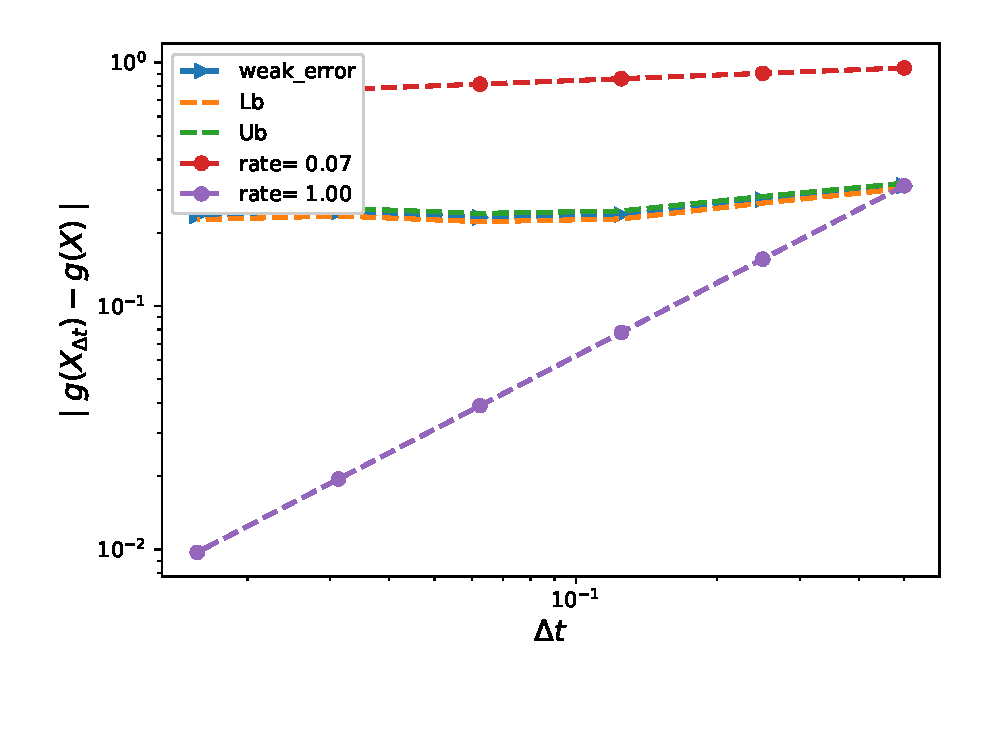
\includegraphics[width=0.4\linewidth]{./figures/basket_call_2d_time_stepping/weak_convergence/weak_convergence_order_basket_option_2d_relative_M_10_4_beta_64}

	\caption{The rate of convergence of the weak error for the two dimensional basket call option with  a number of Laguerre  quadrature points  $\beta=64$ and number of samples for MC $M=10^4$.  }
	\label{fig:Weak_rate_two_dim_basket}
\end{figure}
\FloatBarrier

To investigate the reason of the observed bad behavior of the weak error, we plot the smoothed integrand $I$ for different scenarios of number of time steps $N \in {4,8}$ with respect to different variables (see Figures \ref{fig:integrand_one_dim_N_4} and \ref{fig:integrand_two_dim_N_4} for $N=4$ and  Figures \ref{fig:integrand_one_dim_N_8} and \ref{fig:integrand_two_dim_N_8} for $N=8$).
\FloatBarrier
\begin{figure}
	\begin{subfigure}{.4\textwidth}
		\centering
			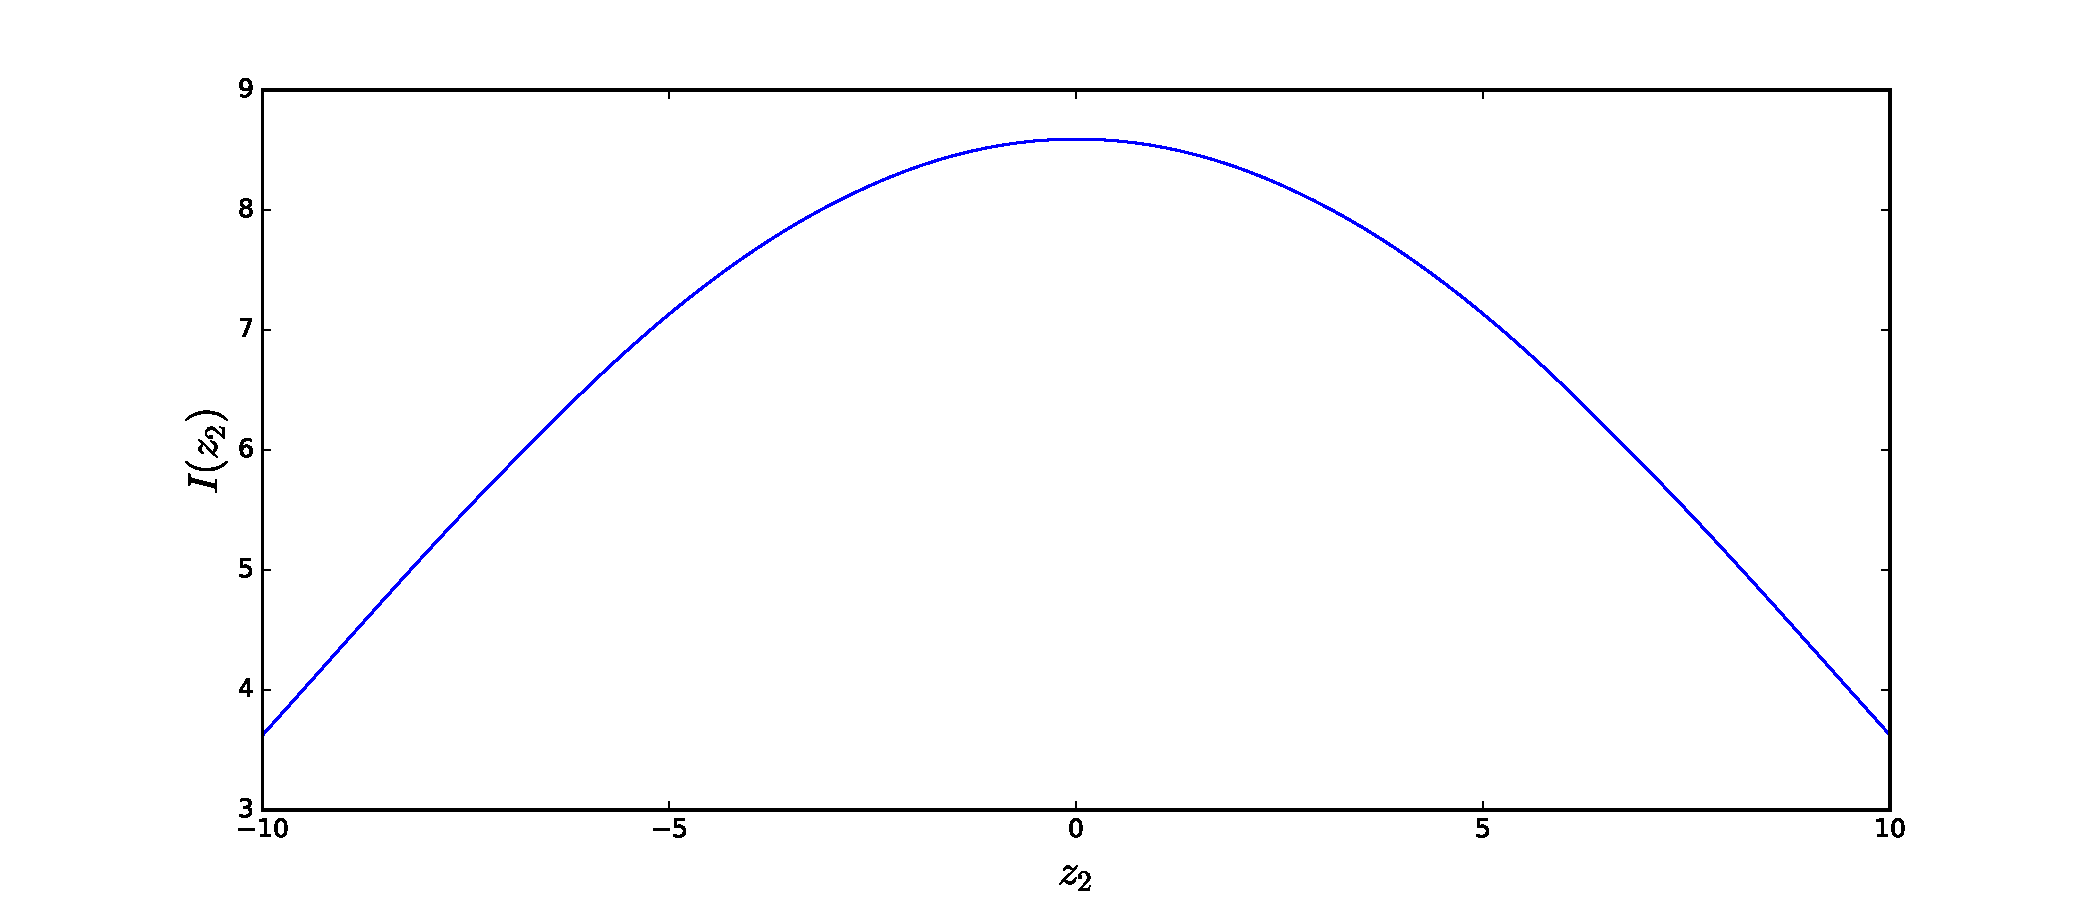
\includegraphics[width=1\linewidth]{./figures/basket_call_2d_time_stepping/integrand_plotting/N_4/1d_plots/smoothed_integrand_basket_2D_N_4_z2}
		\caption{}
	\end{subfigure}%
	\begin{subfigure}{.4\textwidth}
		\centering
			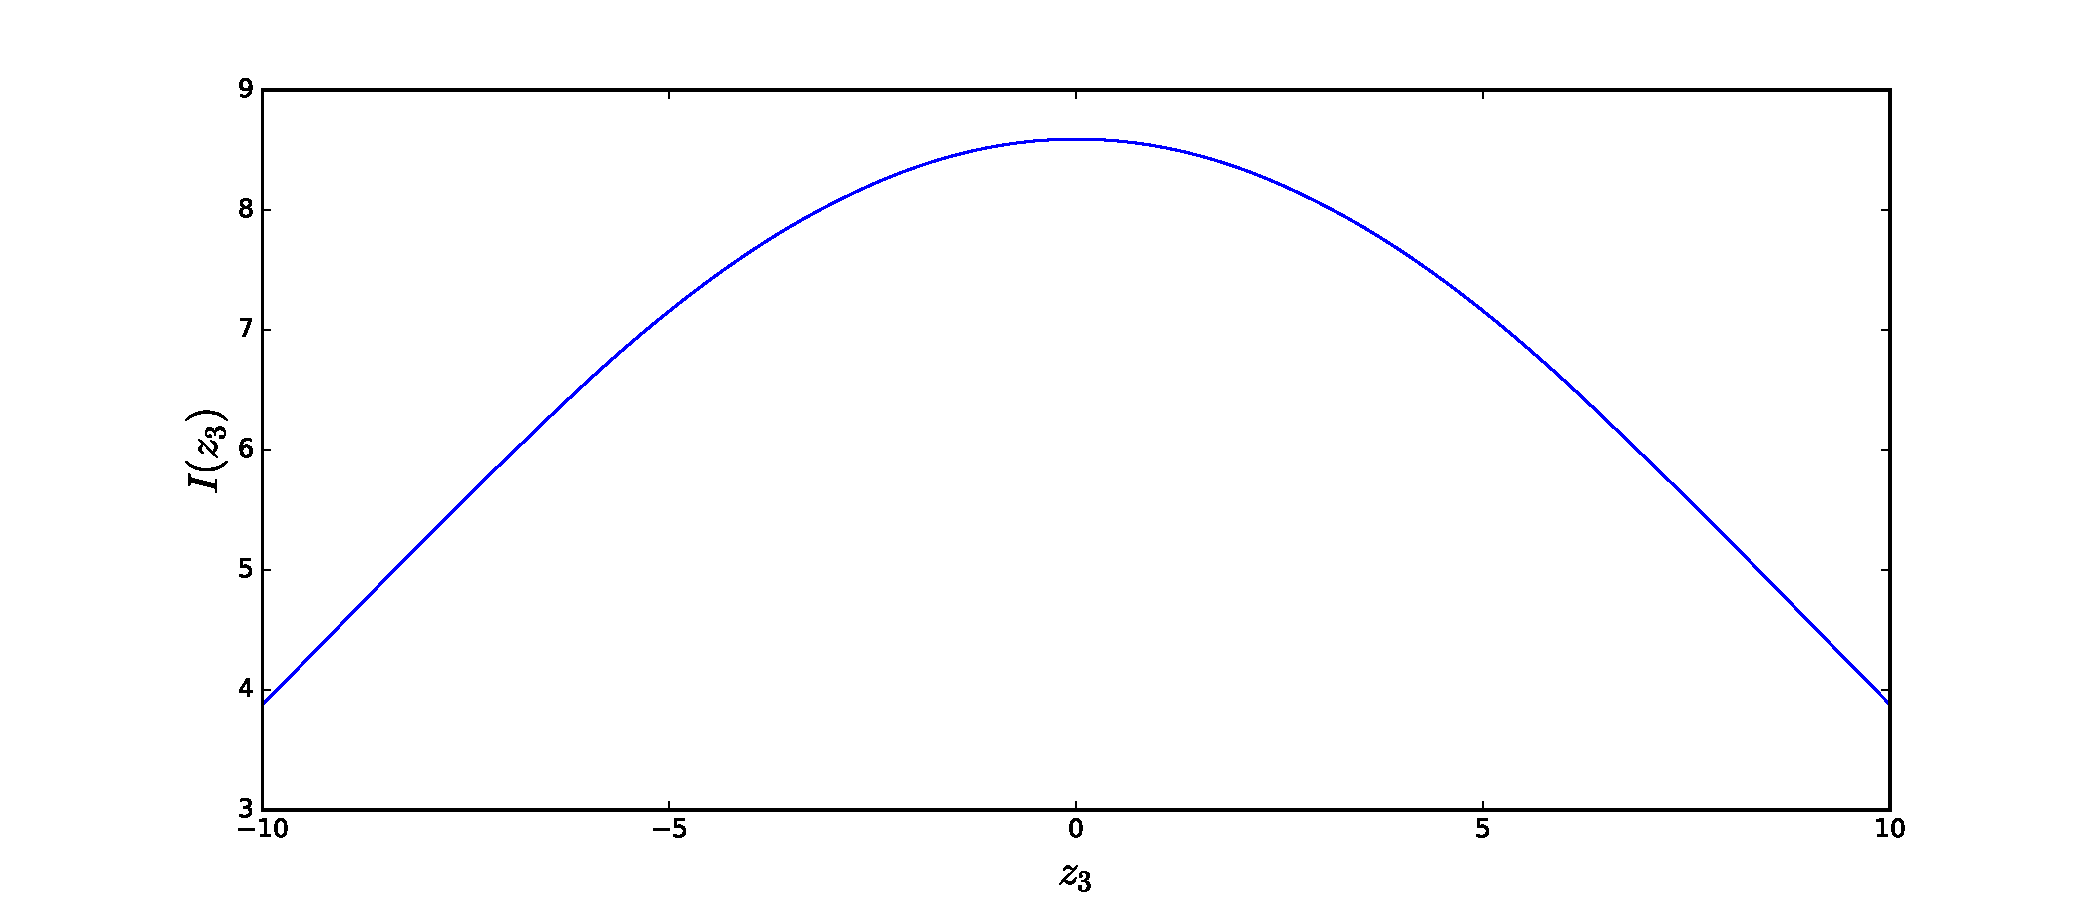
\includegraphics[width=1\linewidth]{./figures/basket_call_2d_time_stepping/integrand_plotting/N_4/1d_plots/smoothed_integrand_basket_2D_N_4_z3}
		\caption{}
	\end{subfigure}\\[1ex]
	\begin{subfigure}{.4\textwidth}
		\centering
			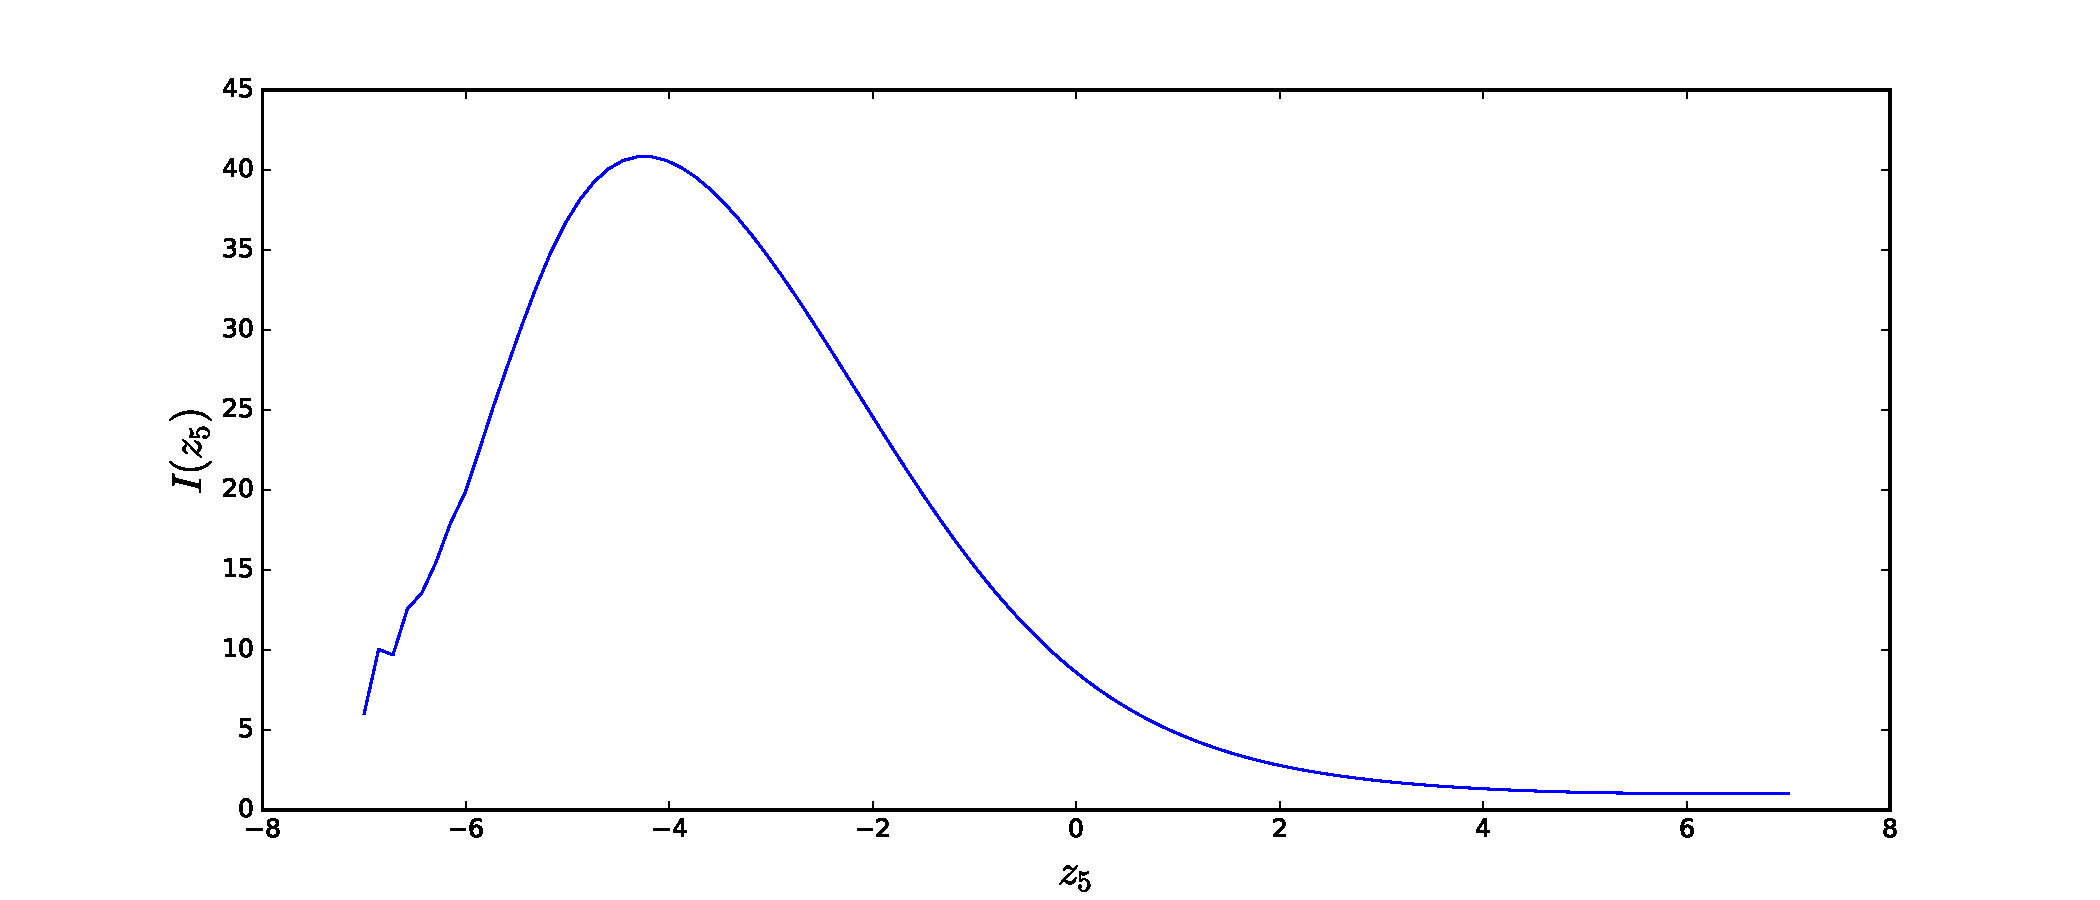
\includegraphics[width=1\linewidth]{./figures/basket_call_2d_time_stepping/integrand_plotting/N_4/1d_plots/smoothed_integrand_basket_2D_N_4_z5}
		\caption{}
	\end{subfigure}%
	\begin{subfigure}{.4\textwidth}
		\centering
			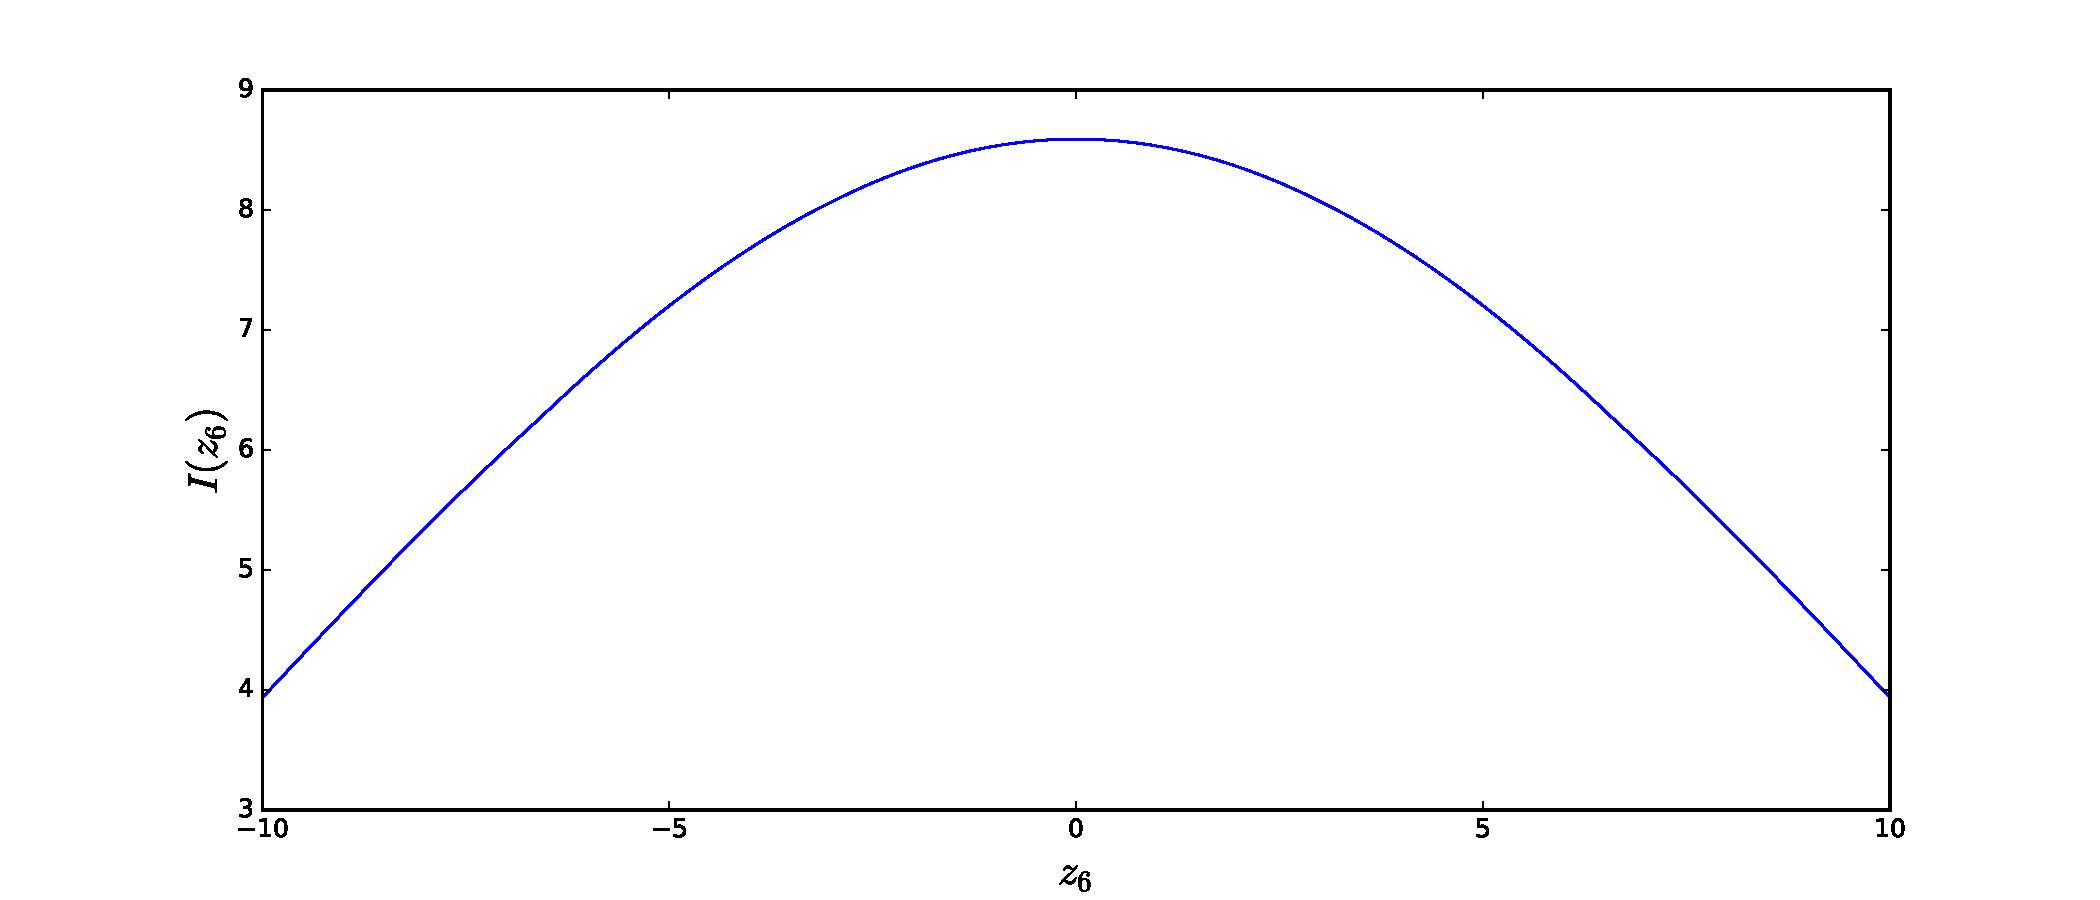
\includegraphics[width=1\linewidth]{./figures/basket_call_2d_time_stepping/integrand_plotting/N_4/1d_plots/smoothed_integrand_basket_2D_N_4_z6}
		\caption{}
		\end{subfigure}
	\caption{The one dimensional plots for the integrand $I$ with respect to the different variables for $N=4$. a) with respect to $z_2$, b) with respect to $z_3$, c) with respect to $z_5$,  d) with respect to $z_6$.}
	\label{fig:integrand_one_dim_N_4}
\end{figure}
\FloatBarrier


\FloatBarrier
\begin{figure}
	\begin{subfigure}{.4\textwidth}
		\centering
			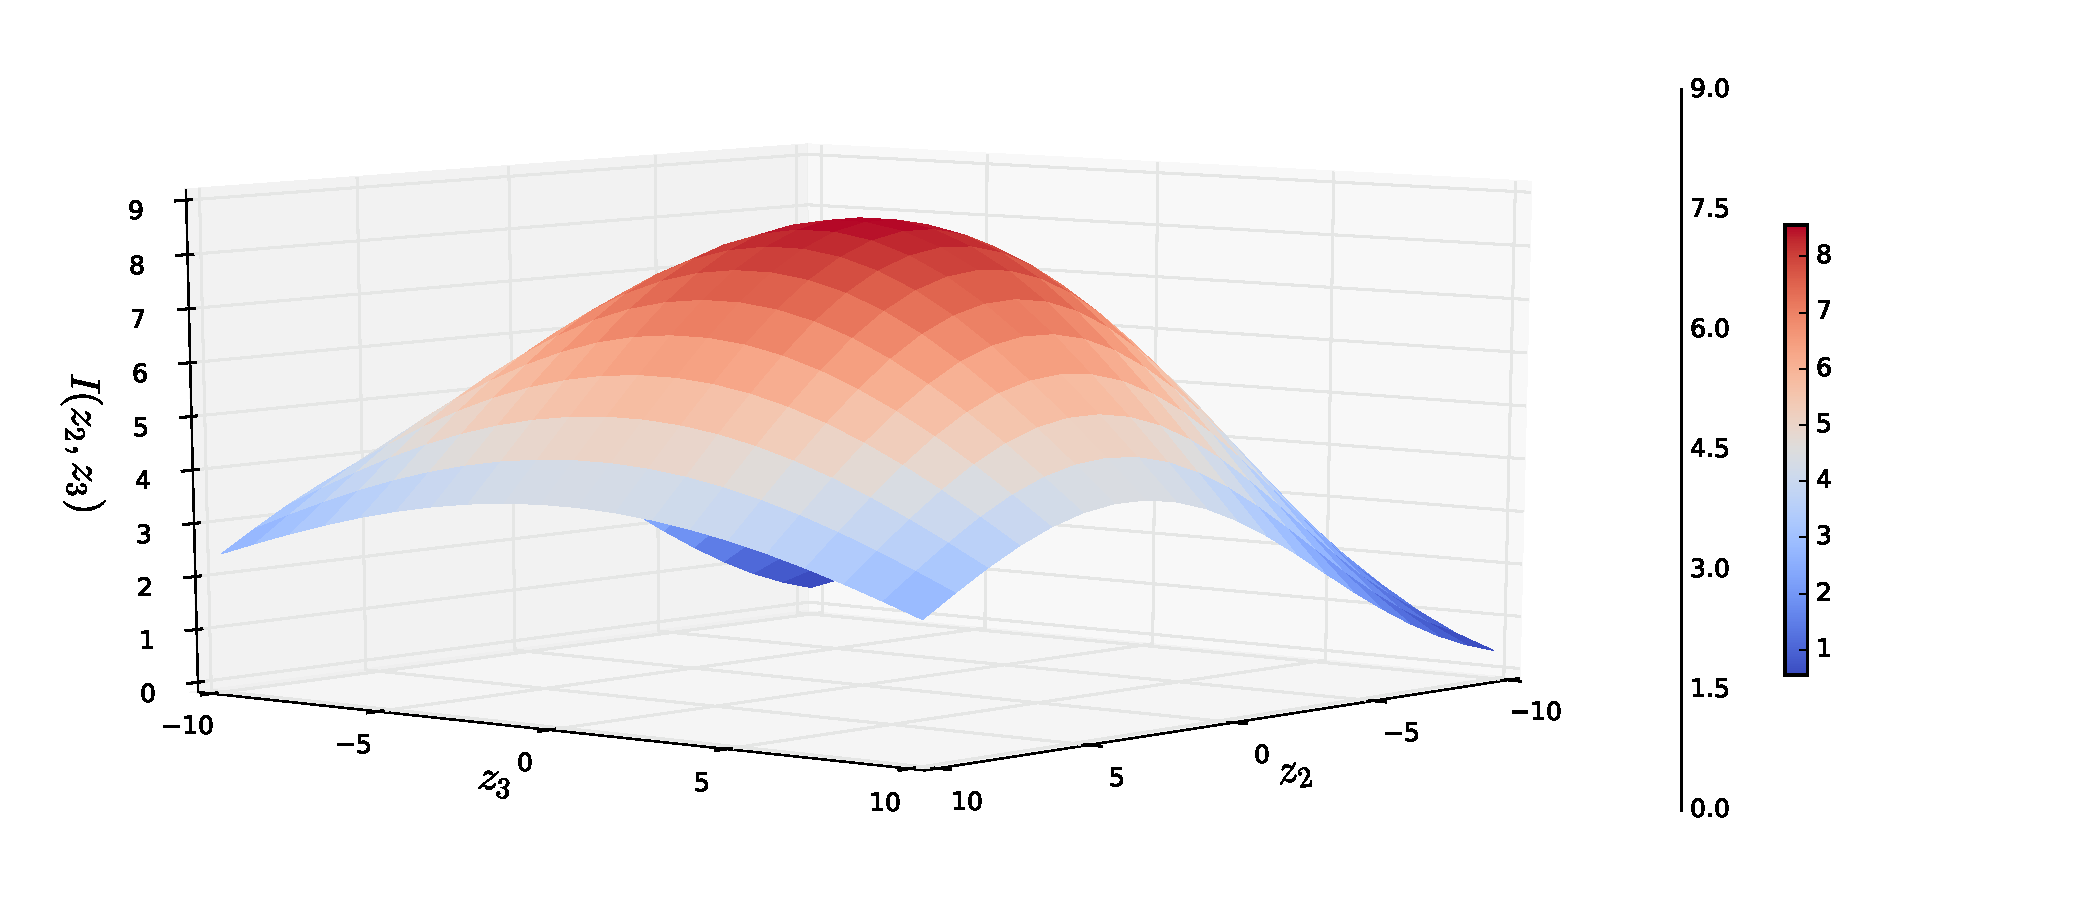
\includegraphics[width=1\linewidth]{./figures/basket_call_2d_time_stepping/integrand_plotting/N_4/2d_plots/z_2_3/smoothed_integrand_basket_2D_N_4_z2_3_40}
		\caption{}
	\end{subfigure}%
	\begin{subfigure}{.4\textwidth}
		\centering
			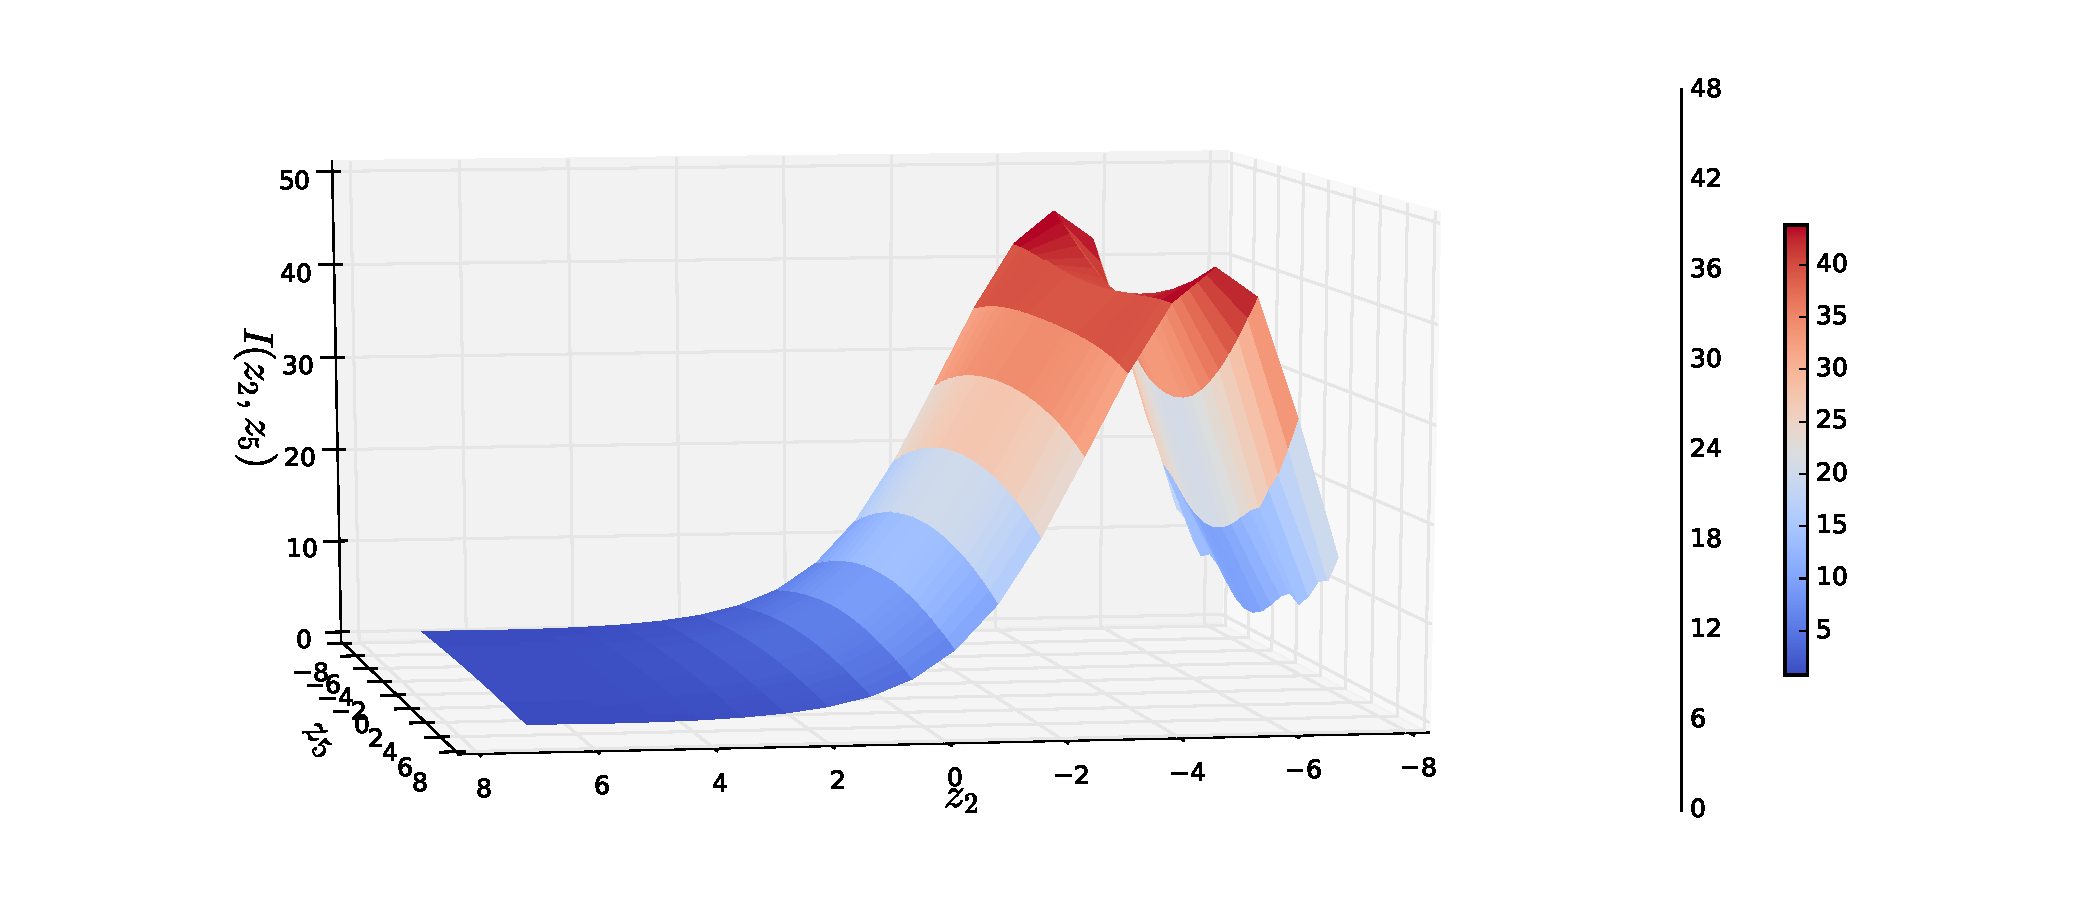
\includegraphics[width=1\linewidth]{./figures/basket_call_2d_time_stepping/integrand_plotting/N_4/2d_plots/z_2_5/smoothed_integrand_basket_2D_N_4_z2_5_80}
		\caption{}
	\end{subfigure}\\[1ex]
	\begin{subfigure}{.4\textwidth}
		\centering
			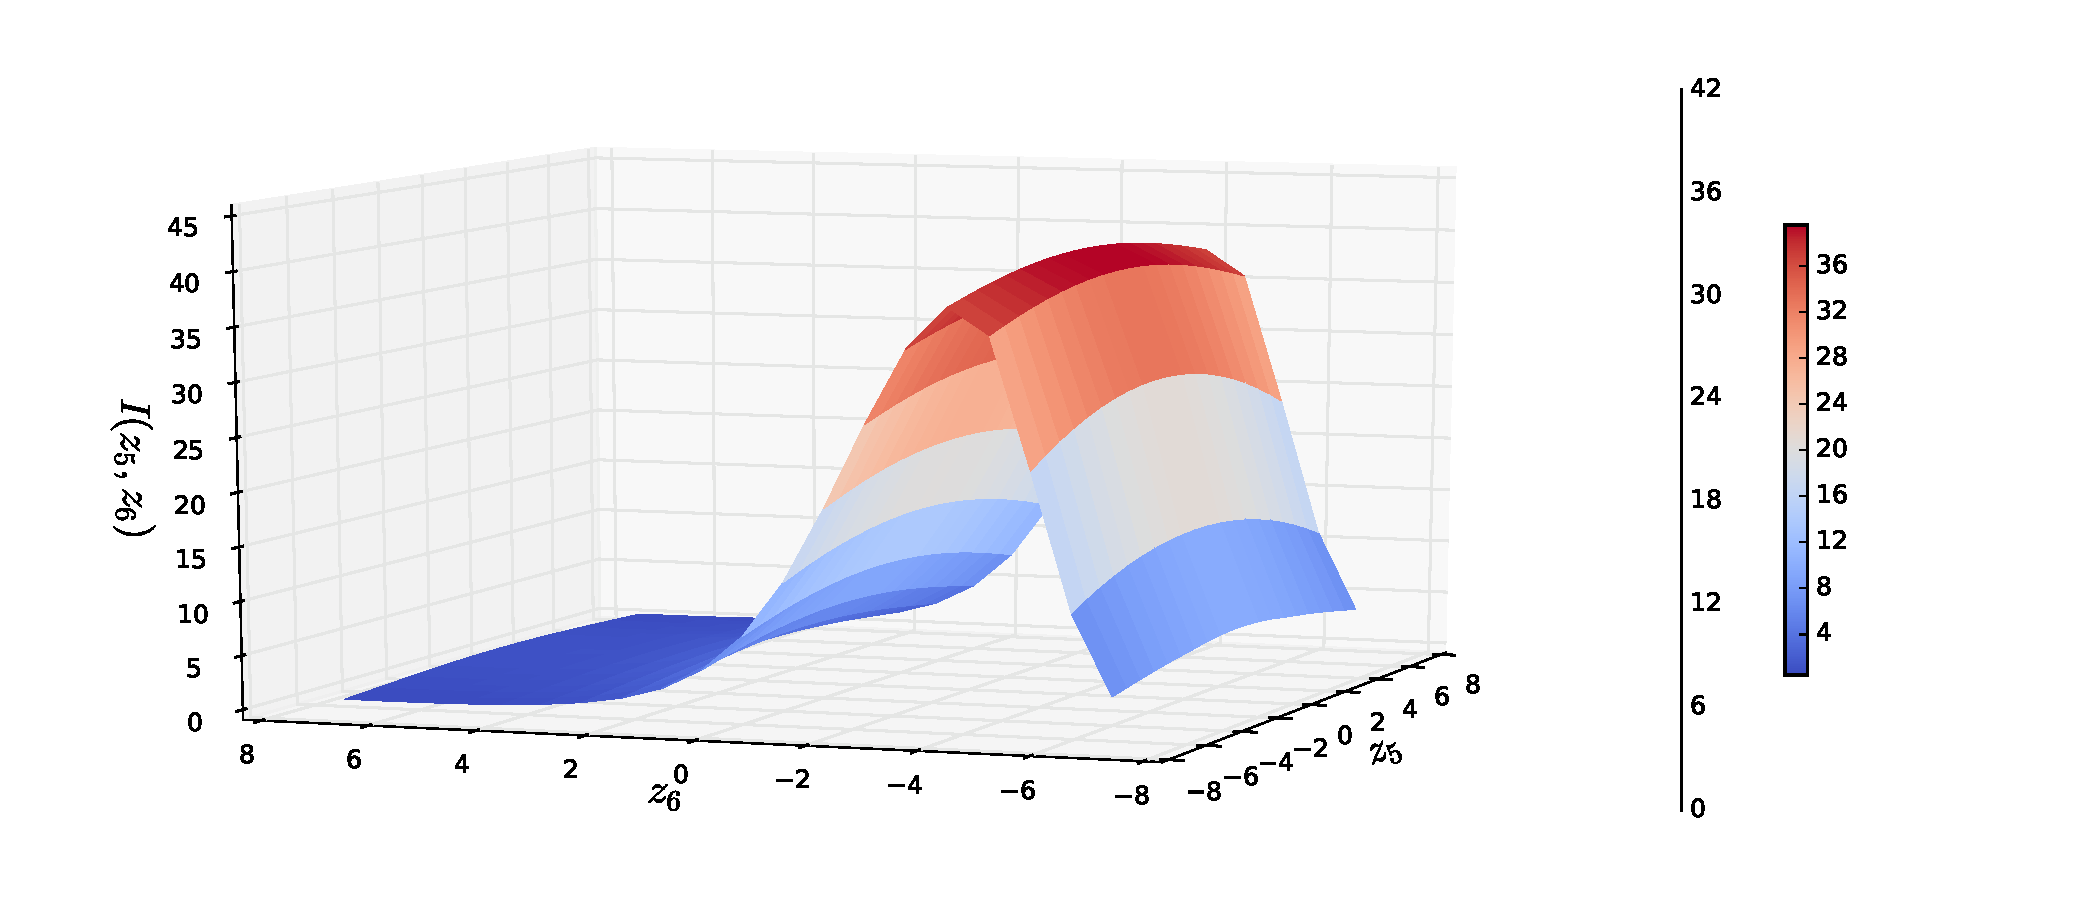
\includegraphics[width=1\linewidth]{./figures/basket_call_2d_time_stepping/integrand_plotting/N_4/2d_plots/z_5_6/smoothed_integrand_basket_2D_N_4_z5_6_200}
		\caption{}
	\end{subfigure}%
	\begin{subfigure}{.4\textwidth}
		\centering
			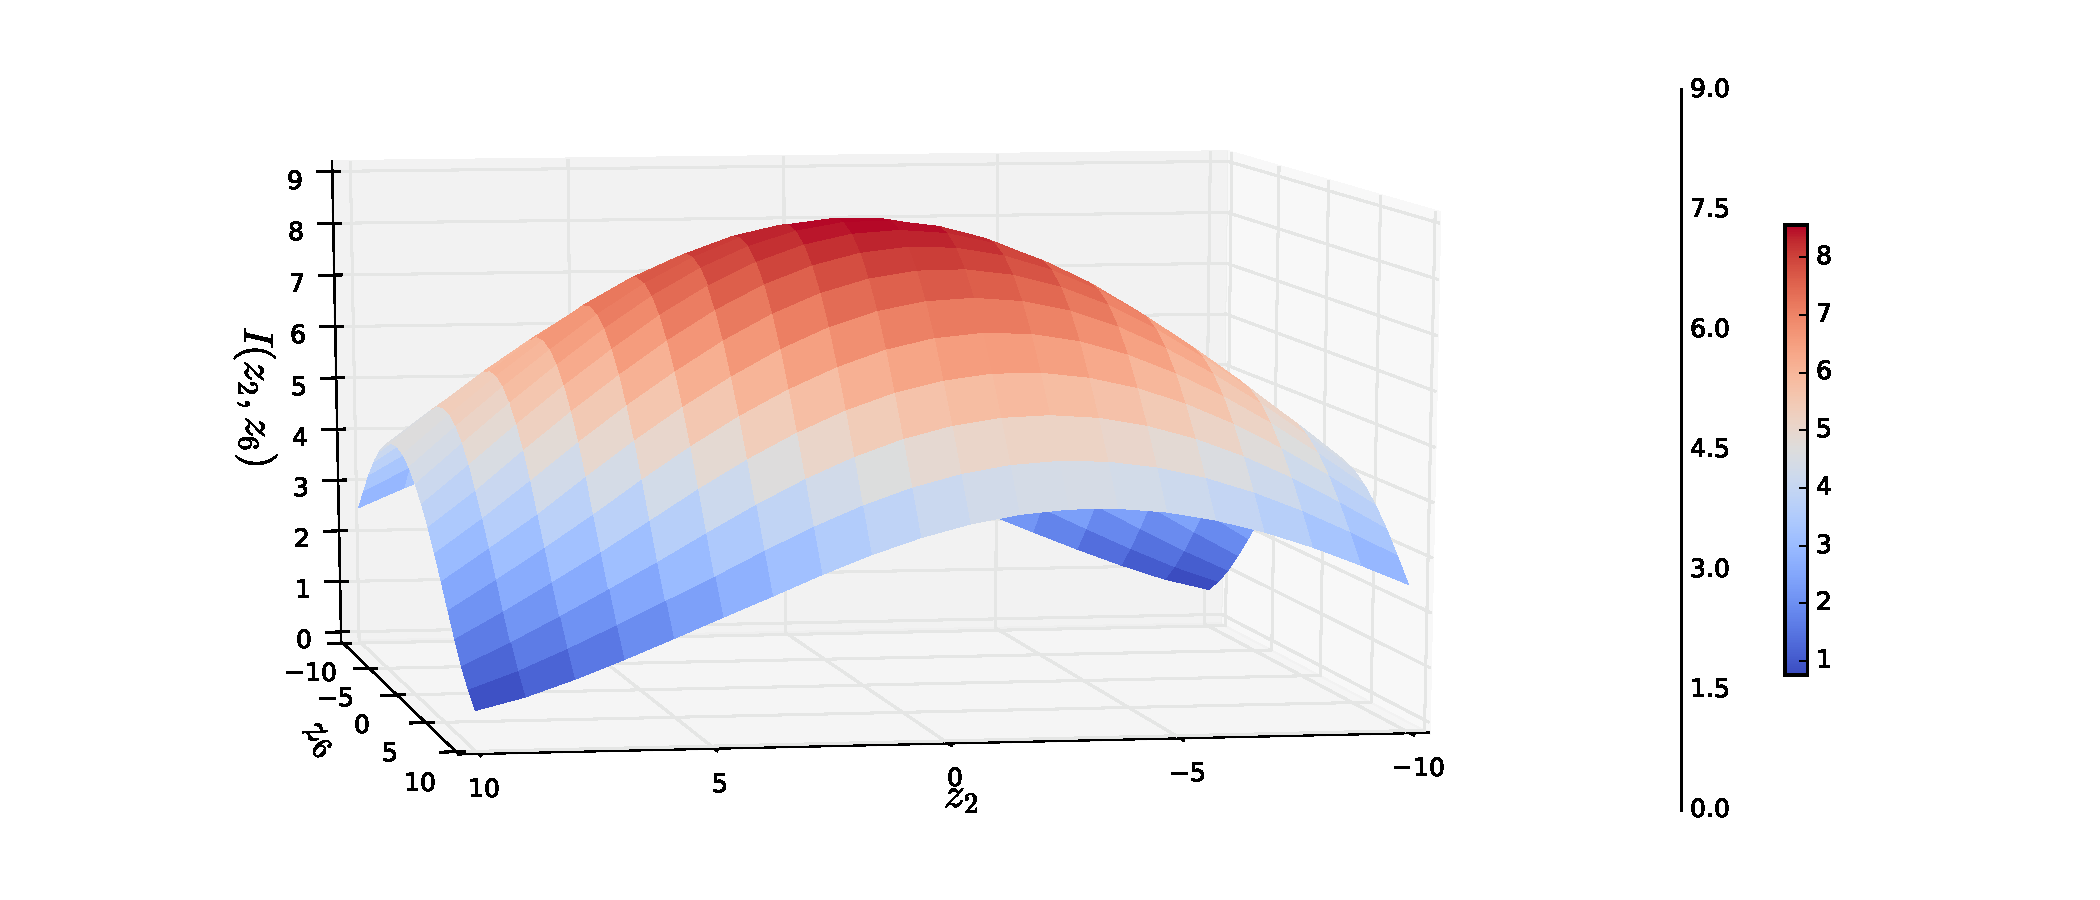
\includegraphics[width=1\linewidth]{./figures/basket_call_2d_time_stepping/integrand_plotting/N_4/2d_plots/z_2_6/smoothed_integrand_basket_2D_N_4_z2_6_80}
		\caption{}
		\end{subfigure}
	\caption{The two dimensional plots for the integrand $I$ with respect to the different variables for $N=4$. a) with respect to $(z_2,z_3)$, b) with respect to $(z_2,z_5)$, c) with respect to $(z_5,z_6)$,  d) with respect to $(z_2,z_6)$.}
	\label{fig:integrand_two_dim_N_4}
\end{figure}
\FloatBarrier
\FloatBarrier
\begin{figure}
	\begin{subfigure}{.4\textwidth}
		\centering
			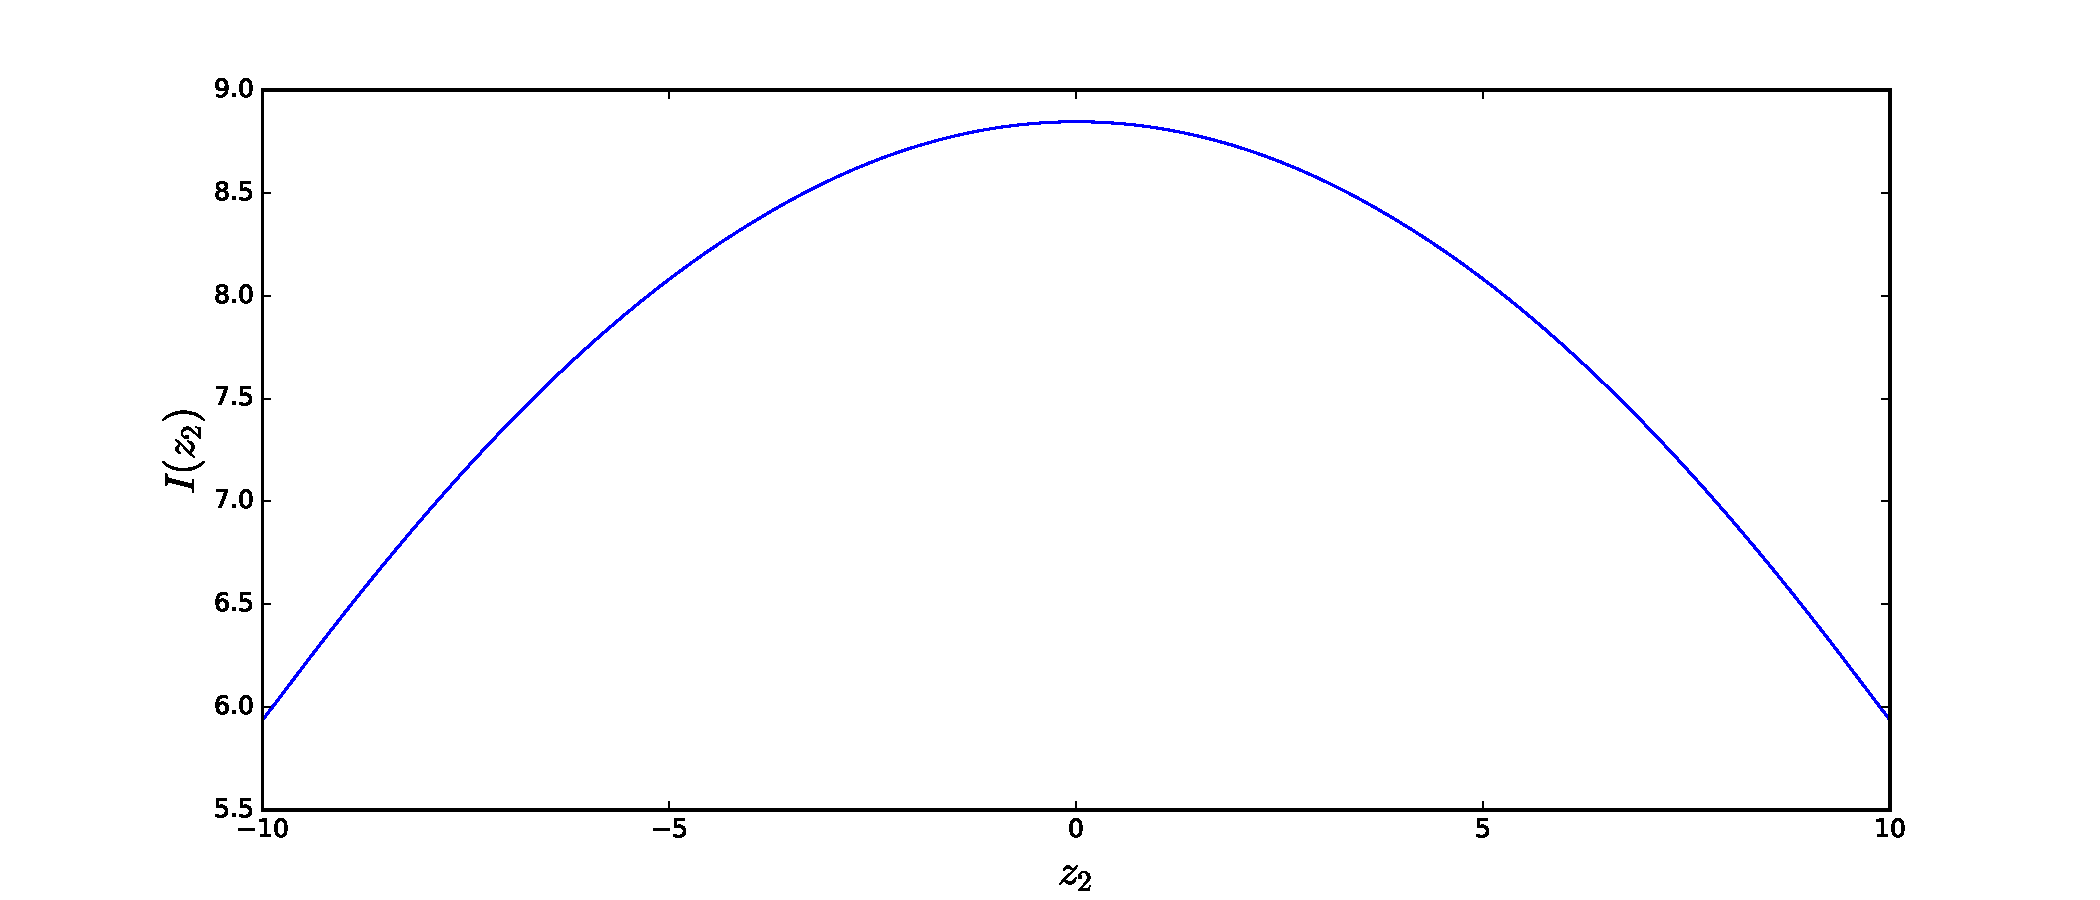
\includegraphics[width=1\linewidth]{./figures/basket_call_2d_time_stepping/integrand_plotting/N_8/1d_plots/smoothed_integrand_basket_2D_N_8_z2}
		\caption{}
	\end{subfigure}%
	\begin{subfigure}{.4\textwidth}
		\centering
			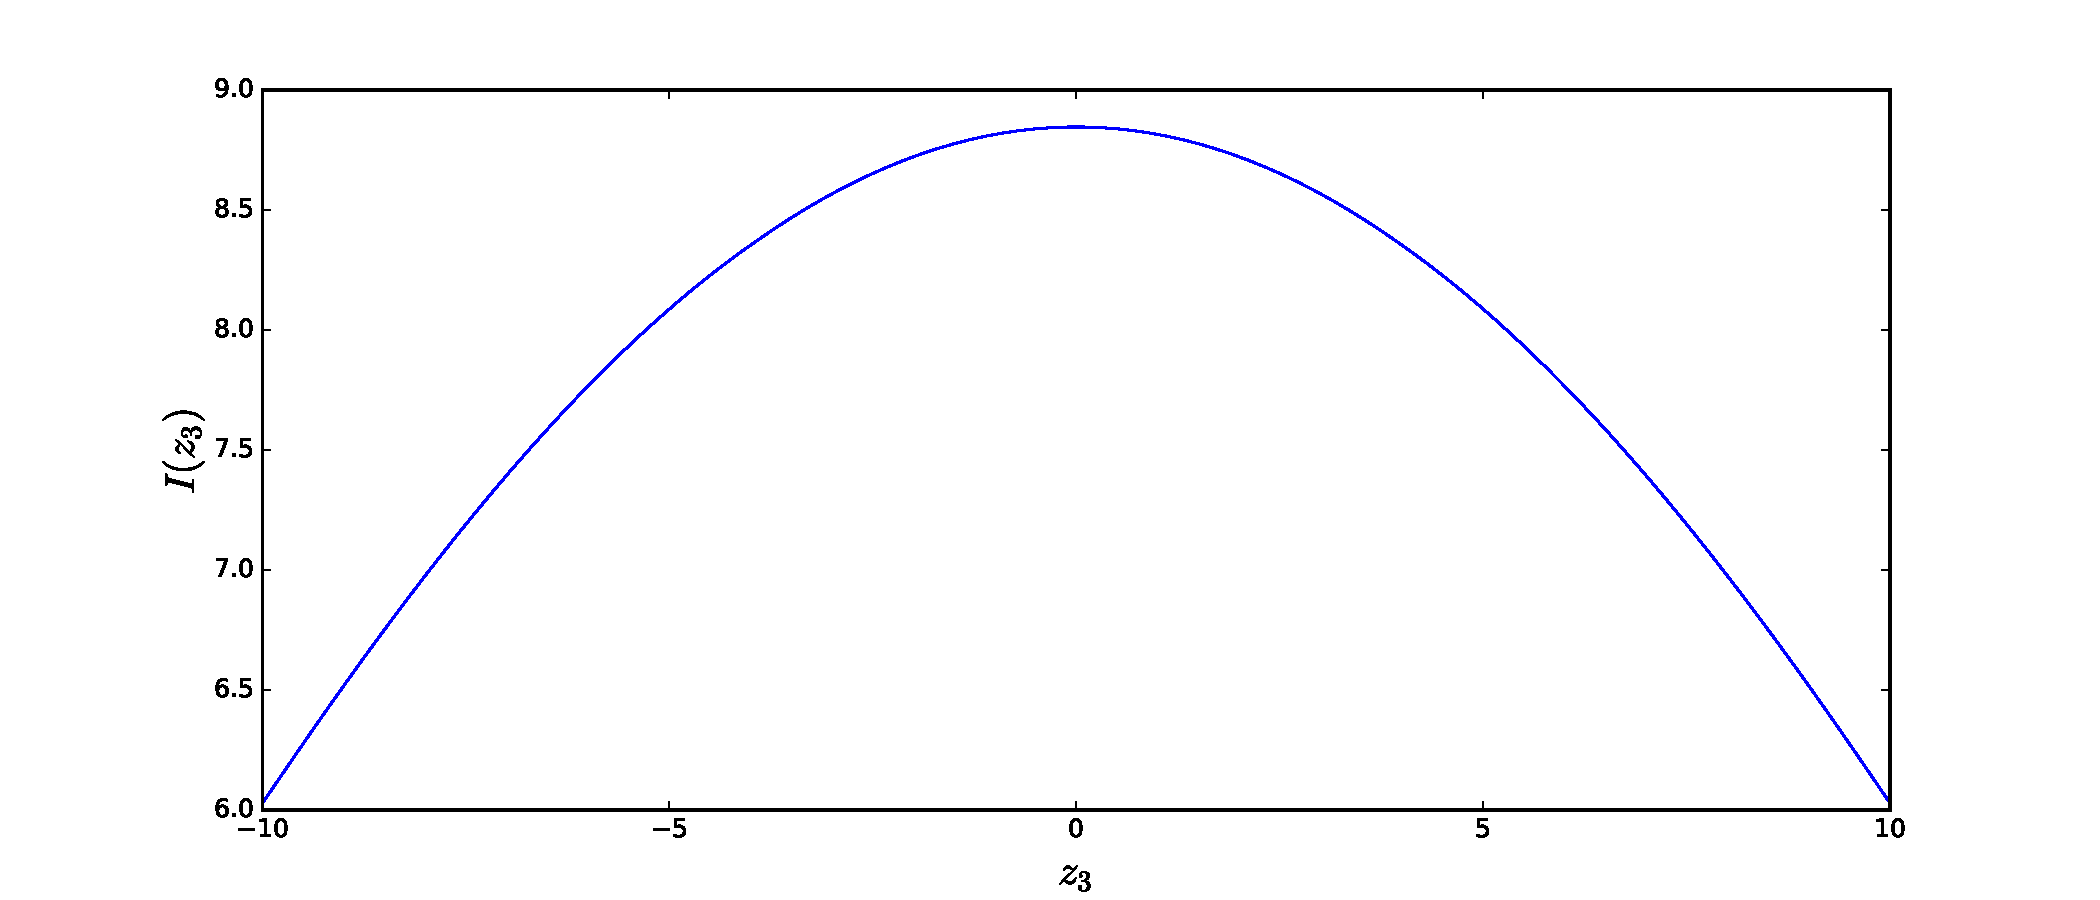
\includegraphics[width=1\linewidth]{./figures/basket_call_2d_time_stepping/integrand_plotting/N_8/1d_plots/smoothed_integrand_basket_2D_N_8_z3}
		\caption{}
	\end{subfigure}\\[1ex]
	\begin{subfigure}{.4\textwidth}
		\centering
			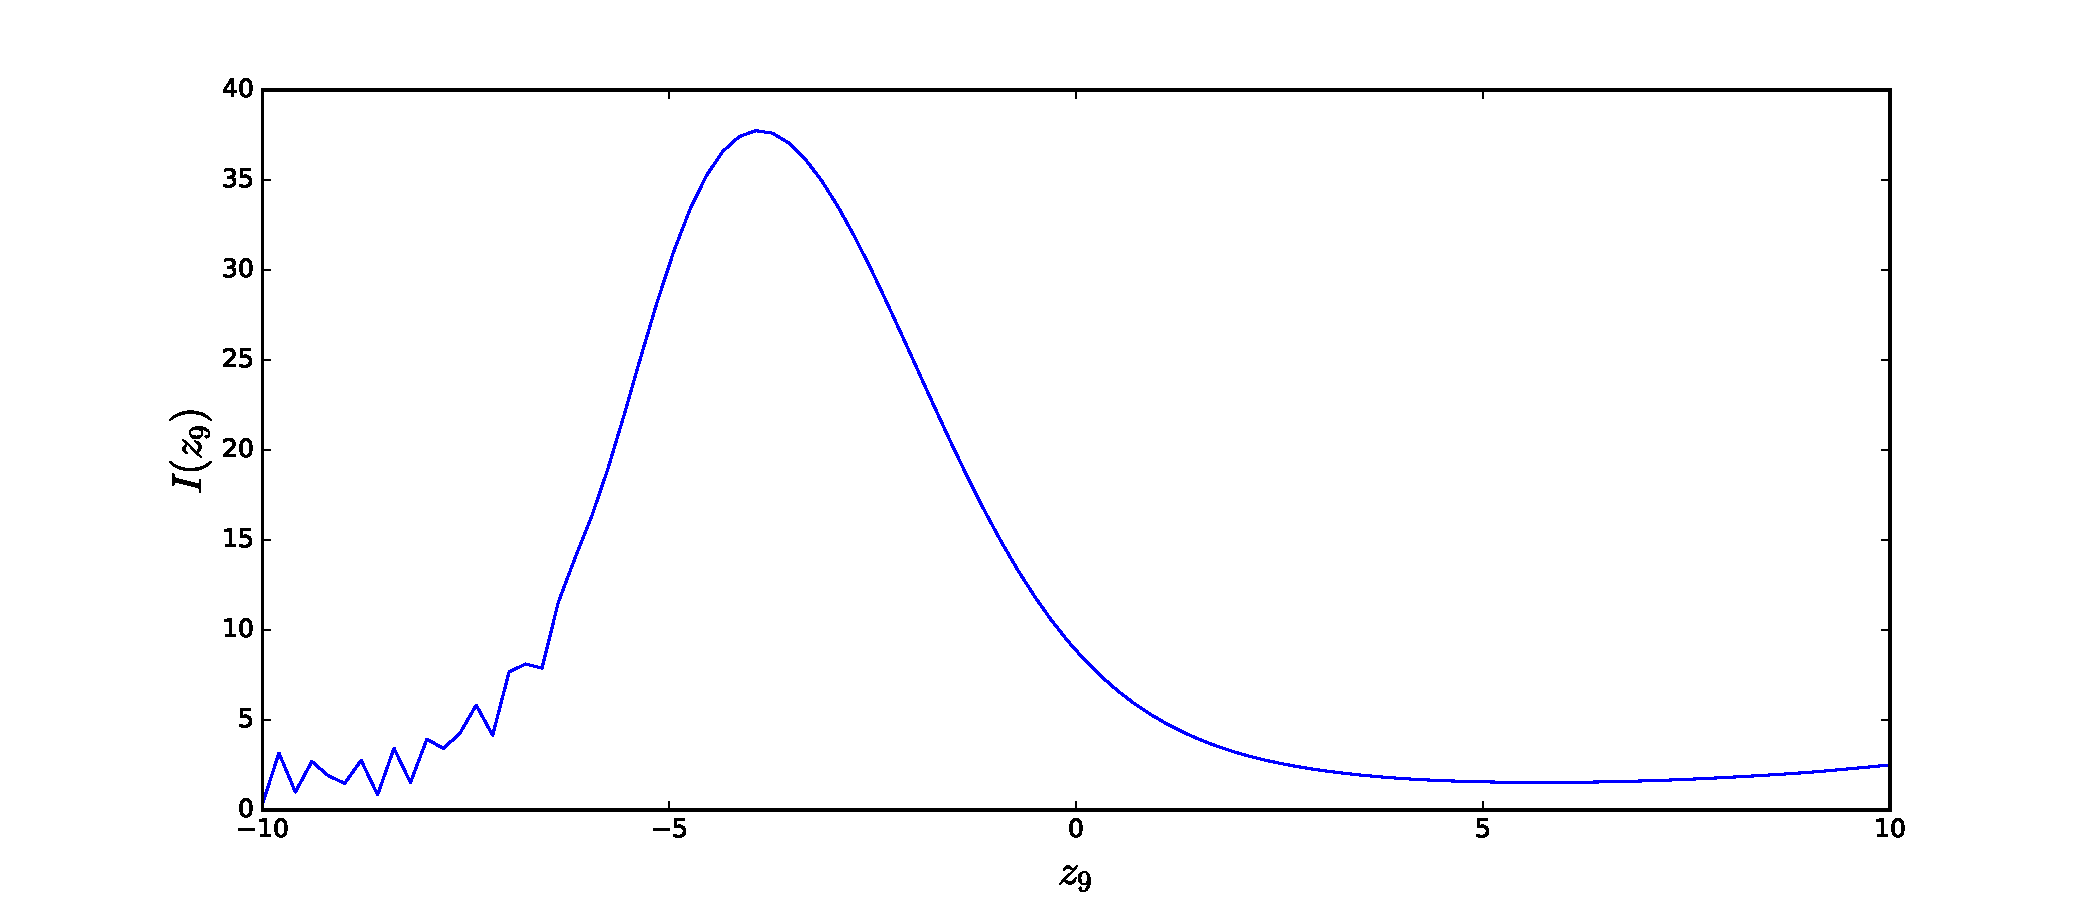
\includegraphics[width=1\linewidth]{./figures/basket_call_2d_time_stepping/integrand_plotting/N_8/1d_plots/smoothed_integrand_basket_2D_N_8_z9}
		\caption{}
	\end{subfigure}%
	\begin{subfigure}{.4\textwidth}
		\centering
			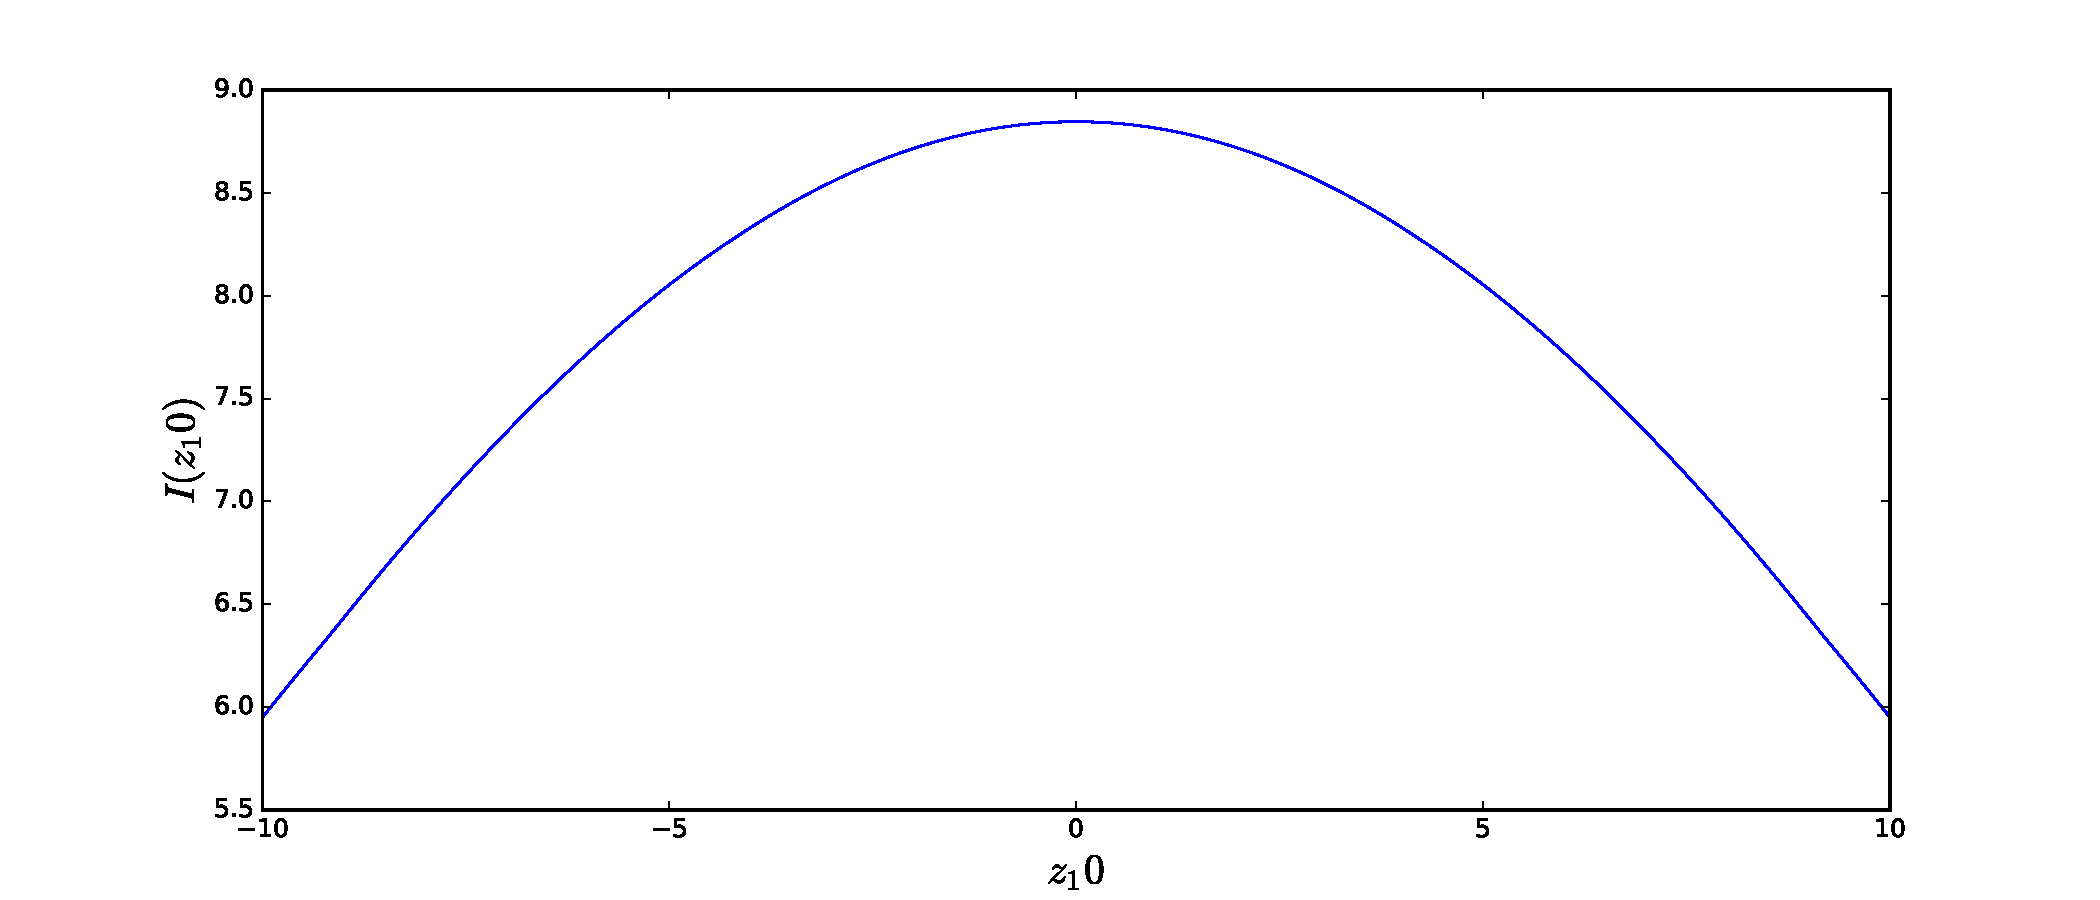
\includegraphics[width=1\linewidth]{./figures/basket_call_2d_time_stepping/integrand_plotting/N_8/1d_plots/smoothed_integrand_basket_2D_N_8_z10}
		\caption{}
		\end{subfigure}
	\caption{The one dimensional plots for the integrand $I$ with respect to the different variables for $N=8$. a) with respect to $z_2$, b) with respect to $z_3$, c) with respect to $z_9$,  d) with respect to $z_10$.}
	\label{fig:integrand_one_dim_N_8}
\end{figure}
\FloatBarrier


\FloatBarrier
\begin{figure}
	\begin{subfigure}{.4\textwidth}
		\centering
			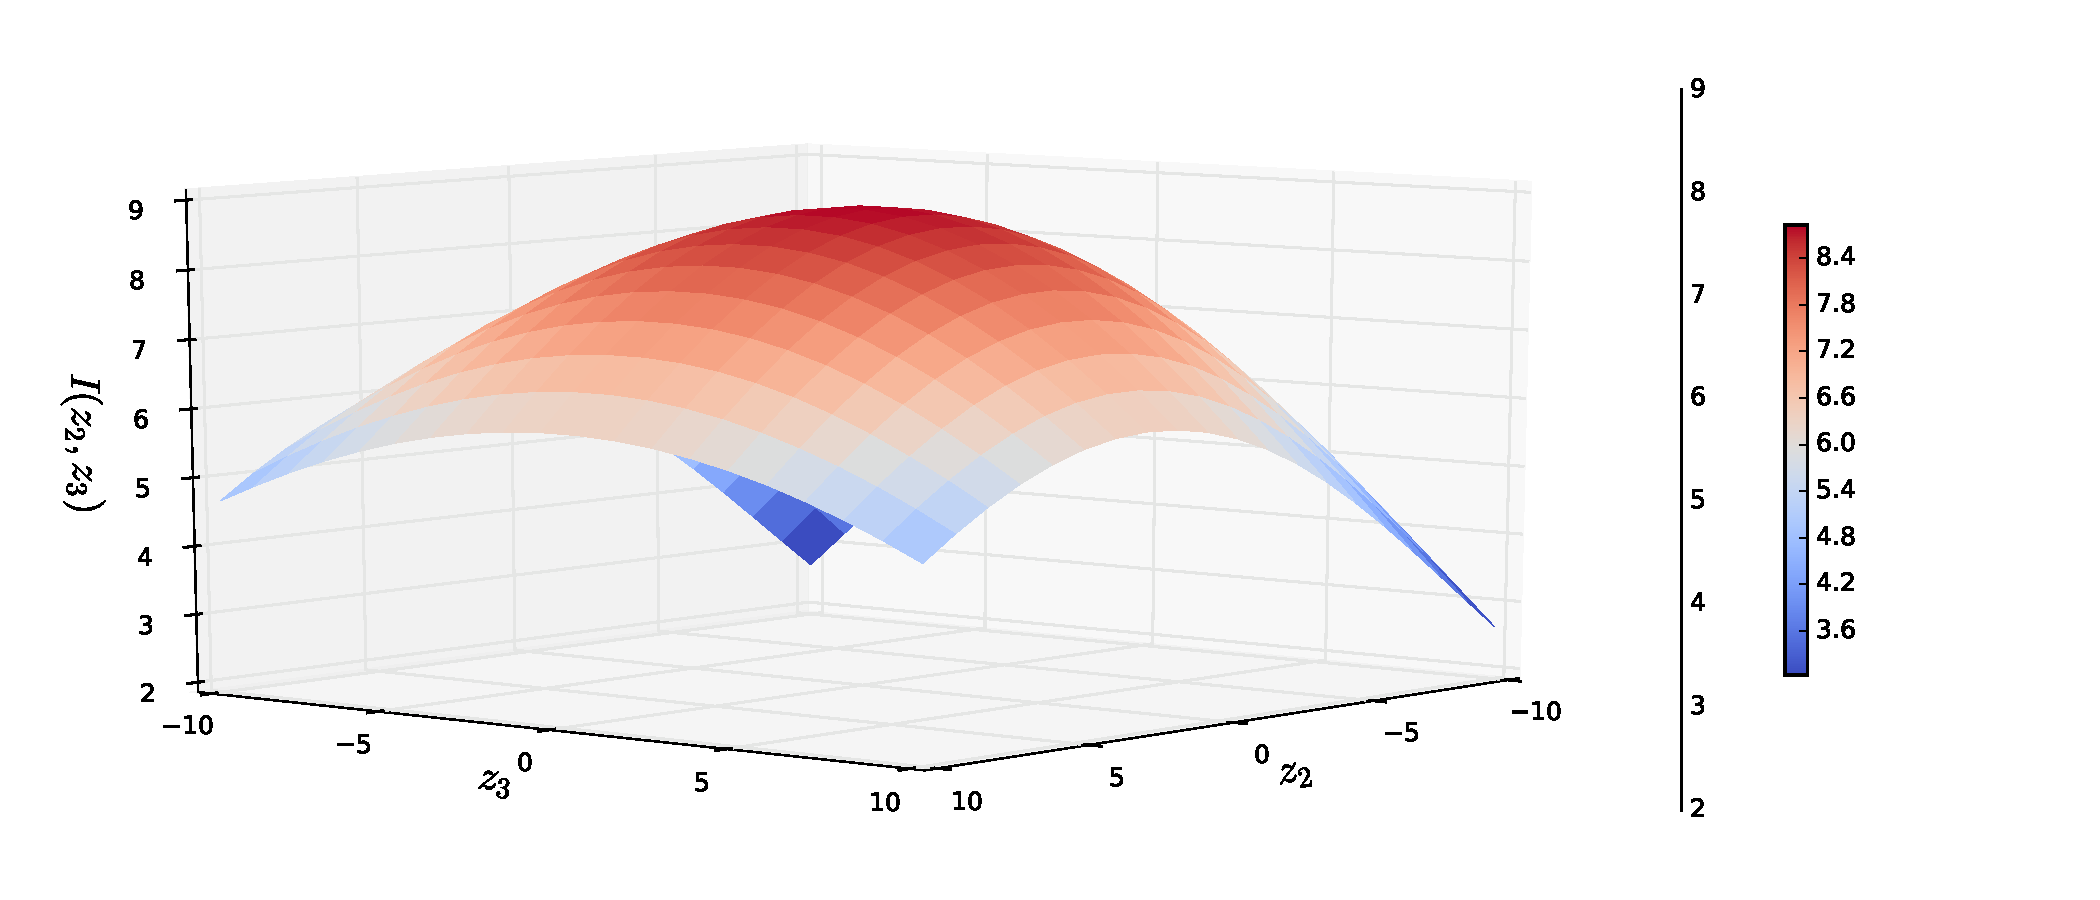
\includegraphics[width=1\linewidth]{./figures/basket_call_2d_time_stepping/integrand_plotting/N_8/2d_plots/z_2_3/smoothed_integrand_basket_2D_N_8_z2_3_40}
		\caption{}
	\end{subfigure}%
	\begin{subfigure}{.4\textwidth}
		\centering
			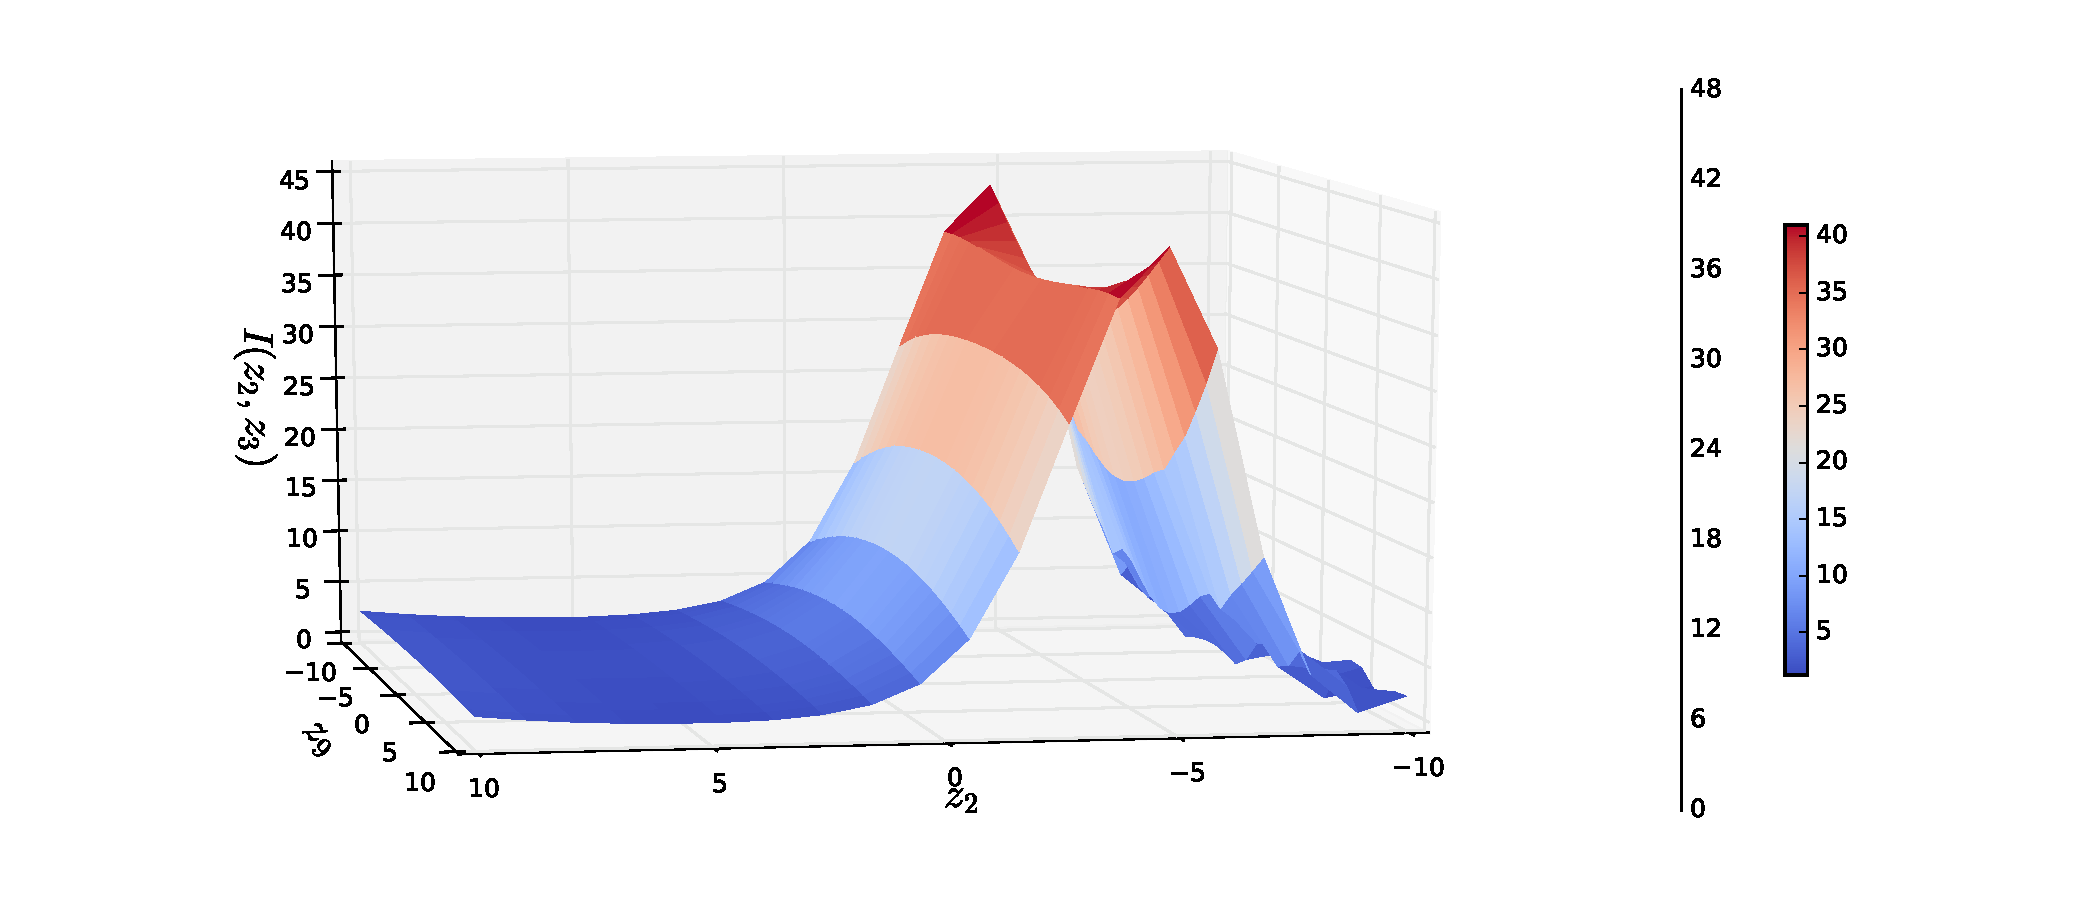
\includegraphics[width=1\linewidth]{./figures/basket_call_2d_time_stepping/integrand_plotting/N_8/2d_plots/z_2_9/smoothed_integrand_basket_2D_N_8_z2_9_80}
		\caption{}
	\end{subfigure}\\[1ex]
	\begin{subfigure}{.4\textwidth}
		\centering
			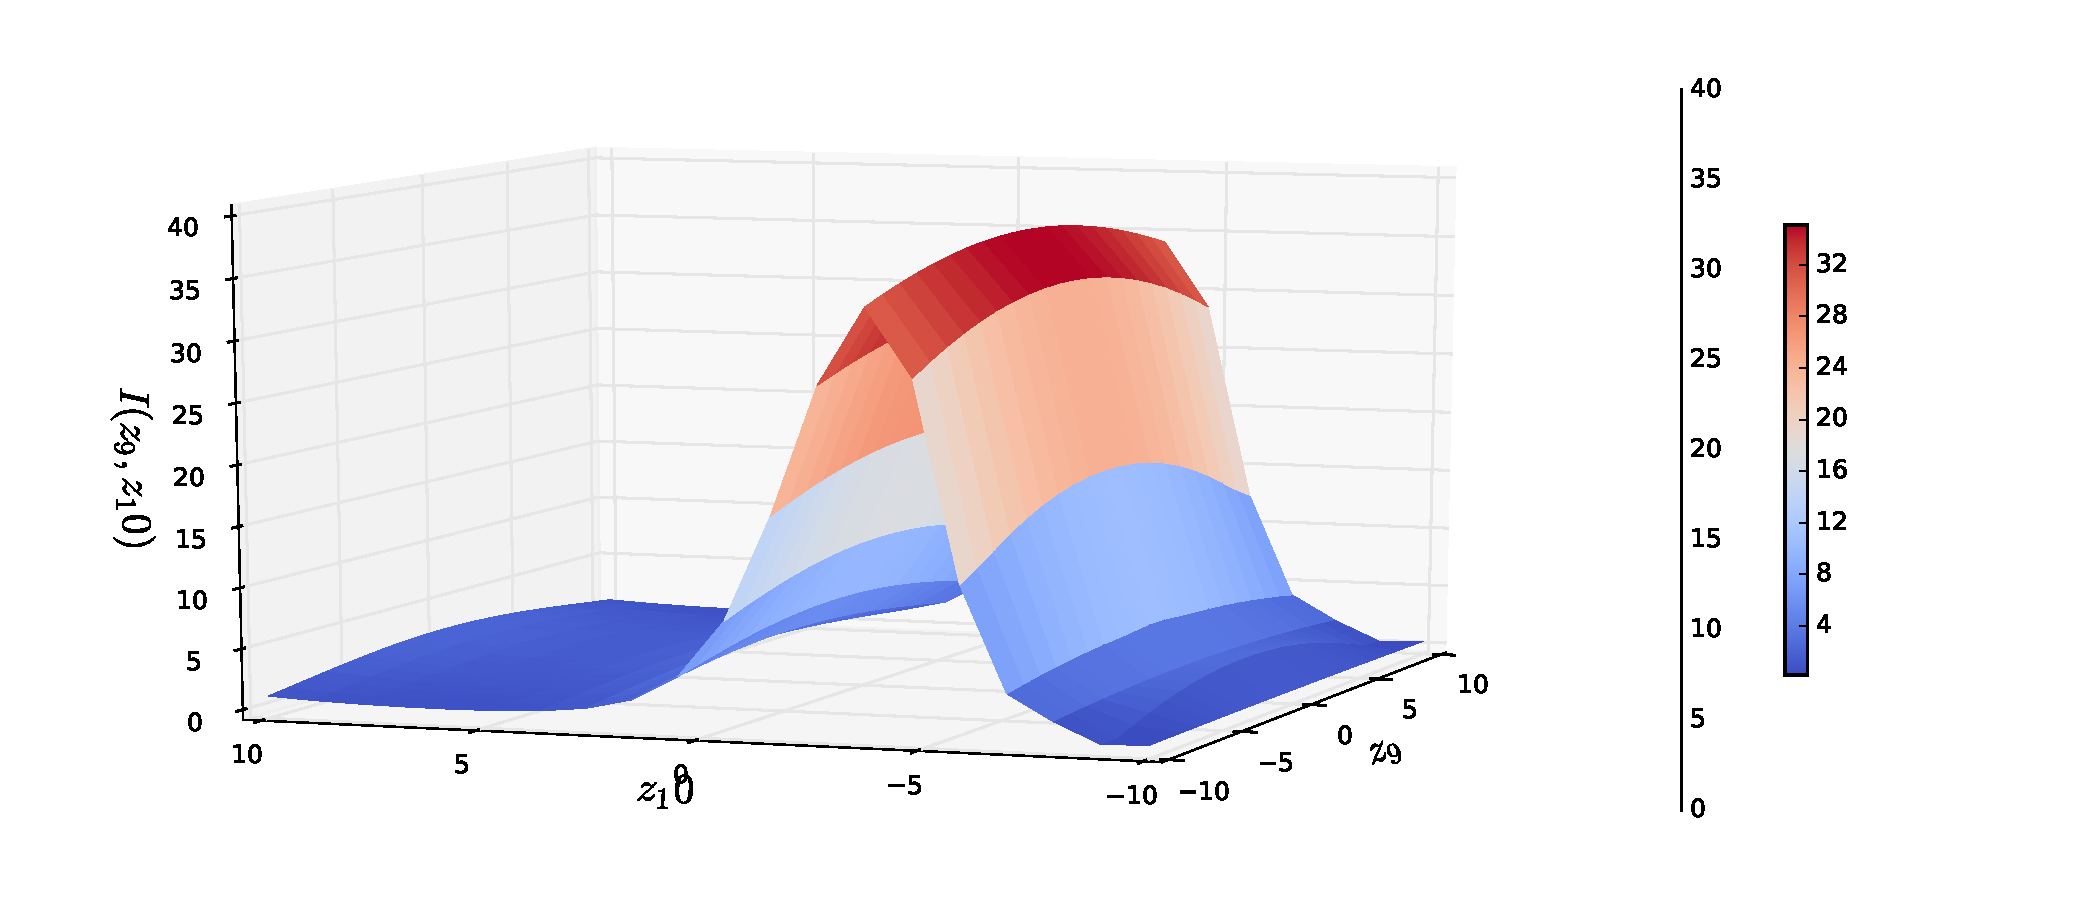
\includegraphics[width=1\linewidth]{./figures/basket_call_2d_time_stepping/integrand_plotting/N_8/2d_plots/z_9_10/smoothed_integrand_basket_2D_N_8_z9_10_200}
		\caption{}
	\end{subfigure}%
	\begin{subfigure}{.4\textwidth}
		\centering
			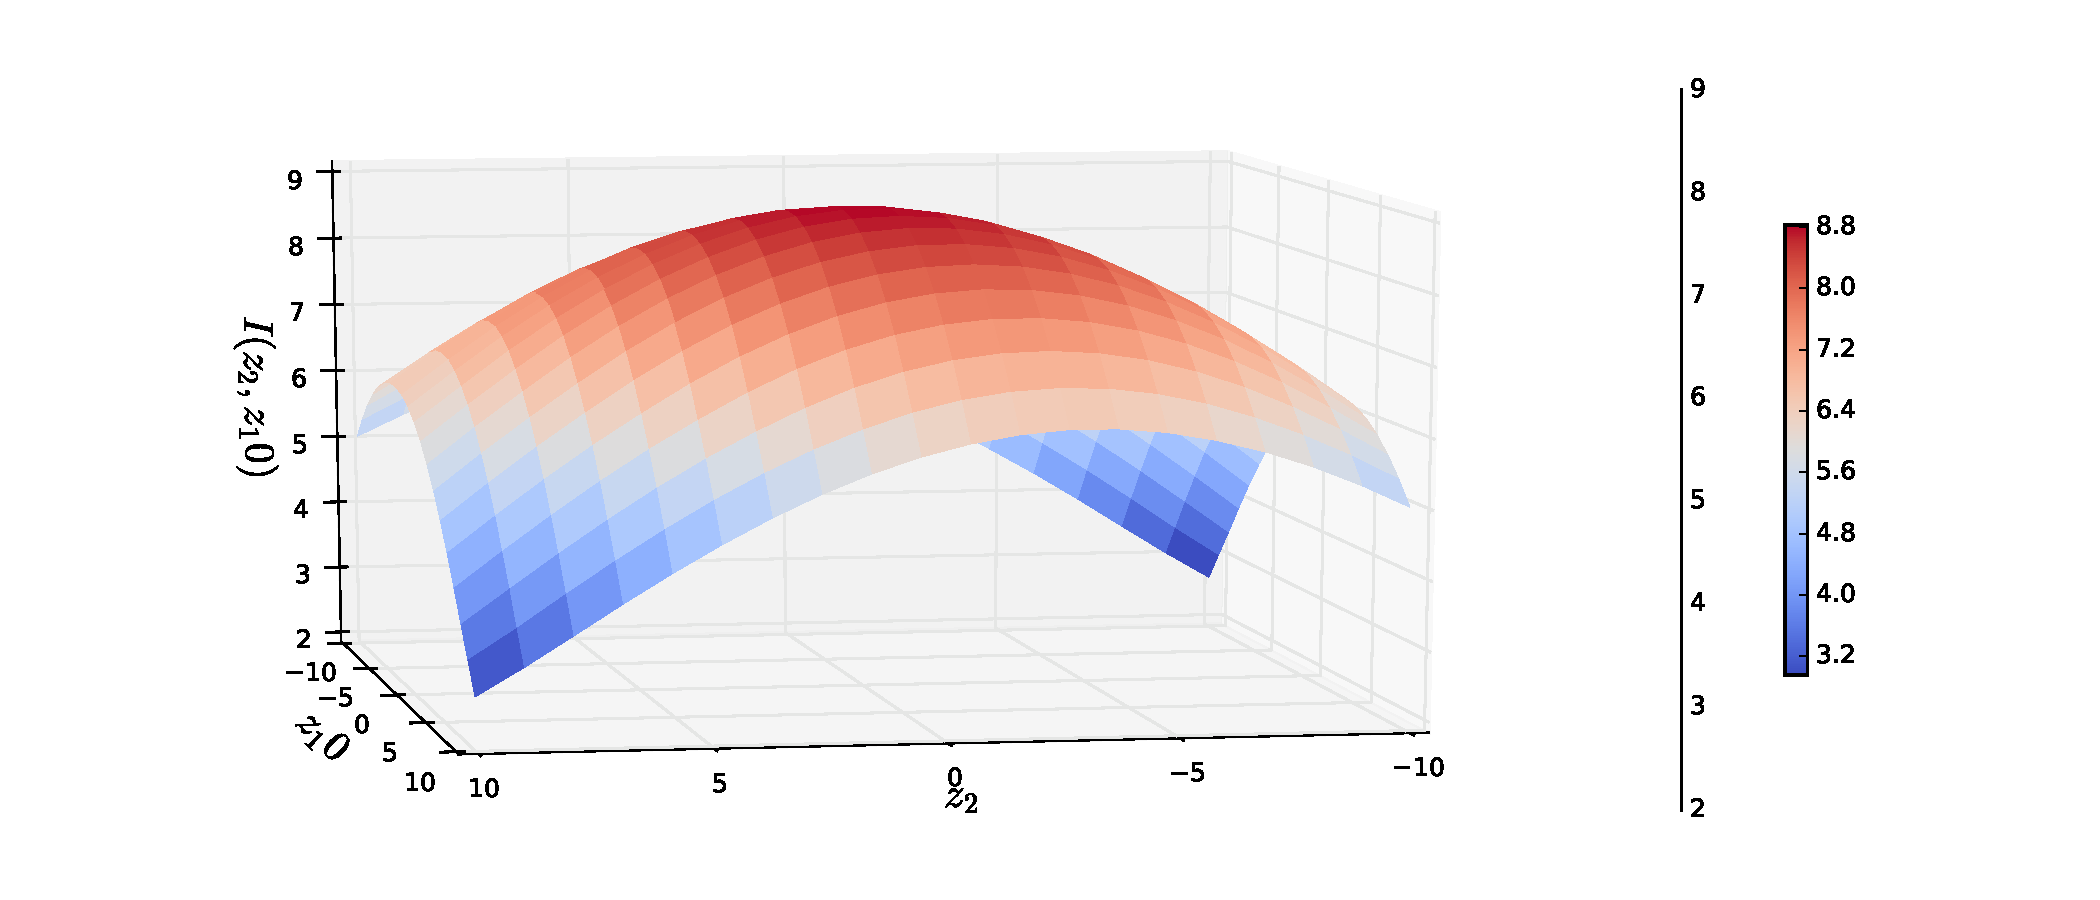
\includegraphics[width=1\linewidth]{./figures/basket_call_2d_time_stepping/integrand_plotting/N_8/2d_plots/z_2_10/smoothed_integrand_basket_2D_N_8_z2_10_80}
		\caption{}
		\end{subfigure}
	\caption{The two dimensional plots for the integrand $I$ with respect to the different variables for $N=8$. a) with respect to $(z_2,z_3)$, b) with respect to $(z_2,z_9)$, c) with respect to $(z_9,z_{10})$,  d) with respect to $(z_2,z_{10})$.}
	\label{fig:integrand_two_dim_N_8}
\end{figure}
\FloatBarrier